% Chapter 2

\chapter{The CMS Detector and Event reconstruction} % Main chapter title

\label{Chapter2_CMS} % For referencing the chapter elsewhere, use \ref{Chapter2_CMS} 
%----------------------------------------------------------------------------------------
%==========================================================================================
Since the data used for the analysis in the dissertation was collected using the CMS detector, this chapter would focus on geometry of CMS, its parts (sub-detectors) and description of how events are reconstructed with the CMS detector.
\section{The Compact Muon Solenoid (CMS) detector}
LHC has set new frontiers for researches in particle physics experiments. State of the art experimental facility has annexed with equipment based on latest technology. To assure the validity of results from the experiment, LHC has its two major and general purpose experiments for cross-validation, one of which is CMS. They have same physics goals with some different design and the detector technology. Particulary the CMS is capable to provide good resolution for muon identification and momentum over wide range of dimensions and determination of the charge on muons with ultimate precision with momentum up to 1~TeV.
It gives healthy inner tacker reconstruction efficiency and resolution of charged particle momentum. It has efficient trigger system and better discrimination of  $\tau$'s and b-jets. Further, it is benefitted from good dielectron, diphoton and dijet mass and energy resolutions, and as well as missing-transverse-energy (MET) resolutions. 
This makes it capable to study large areas from SM Physics (including Higgs Physics) to search for extra dimensions and the dark matter covering physics in energy range from a few 100~GeV to TeV scale~\cite{Reference34}.
\subsection{General aspects and the geometry}
Being one of the two general purpose detectors installed at LHC ring, CMS is is constructed in cylinderical shape having length about 28 m and outer ratdius of around 7 m. Its overall height is about 15 m with overall weight of about 14,000 tonnes. Overall deisgn of the CMS detector can been seen in the Figure ~\ref{Fig:CMS_detector_design}. 
Learning from the earlier experiment at CERN, CMS engineered to be built in different slices at surface instead of doing everything underground.  And fifteen separate slices were then lowered to underground to be fixed at the LHC tunnel.\par
Moving radially outwards from interaction point of beams, there are inner tracker system (ITS), electromagnetic calorimeter (ECAL) and hadronic calorimeter(HCAL) sub-detectors of CMS which are fitted inside the large solenoid magnet. Inner tracker of CMS have large track multiplicity as being closest to beam pipe where collisions happens.
ECAL is build with crystals of lead tungstate which covers pseudorapidity up to $|\eta| < 3.0$. After ECAL, hadronic calorimeter is installed which is made of brass. Outermost layer of the CMS detector is the Muon System. Details of sub-detectors, trigger system and data acquisition systems will be described in next Sections.
%CMS and ATLAS experiment shares the same physics goal though both independent experiment uses different technical solution and detectors design. It is apparent from Figure \ref{Fig:lhc_all} that the total cross section proton-proton collisionis at  $\sqrt{s} = 14 $~TeV is approximately 100~mb. While designed LHC luminosity leads to have $10^9$ inelastic events/s approximately. It is huge experimental challenge to deal with such high rate collisions. 
%CMS trigger system helps to select online events and reducing the huge rate to approximately 100 events/s to be stored and used for physics analysis later. 
%The read-out and trigger system designed to meet the short bunch crossing time, 25 ns. 
%\\Being CMS as general purpose detector, followings are  the main requirements to fulfill physics goal of LHC:
%\begin{itemize}
% \item Good resolution for muon identification and momentum over wide range of dimensions and determination of the charge on muons with ultimate precision with momentum up to 1~TeV.
% \item Healthy inner tacker reconstruction efficiency and resolution of charged particle momentum. Efficient trigger system and better discrimination of  $\tau$'s and b-jets.  
% \item Good dielectron and diphoton mass and energy resolutions. 
% \item Good dijet-mass and missing-transverse-energy (MET) resolutions . 
\end{itemize}
\begin{figure}
\begin{center}
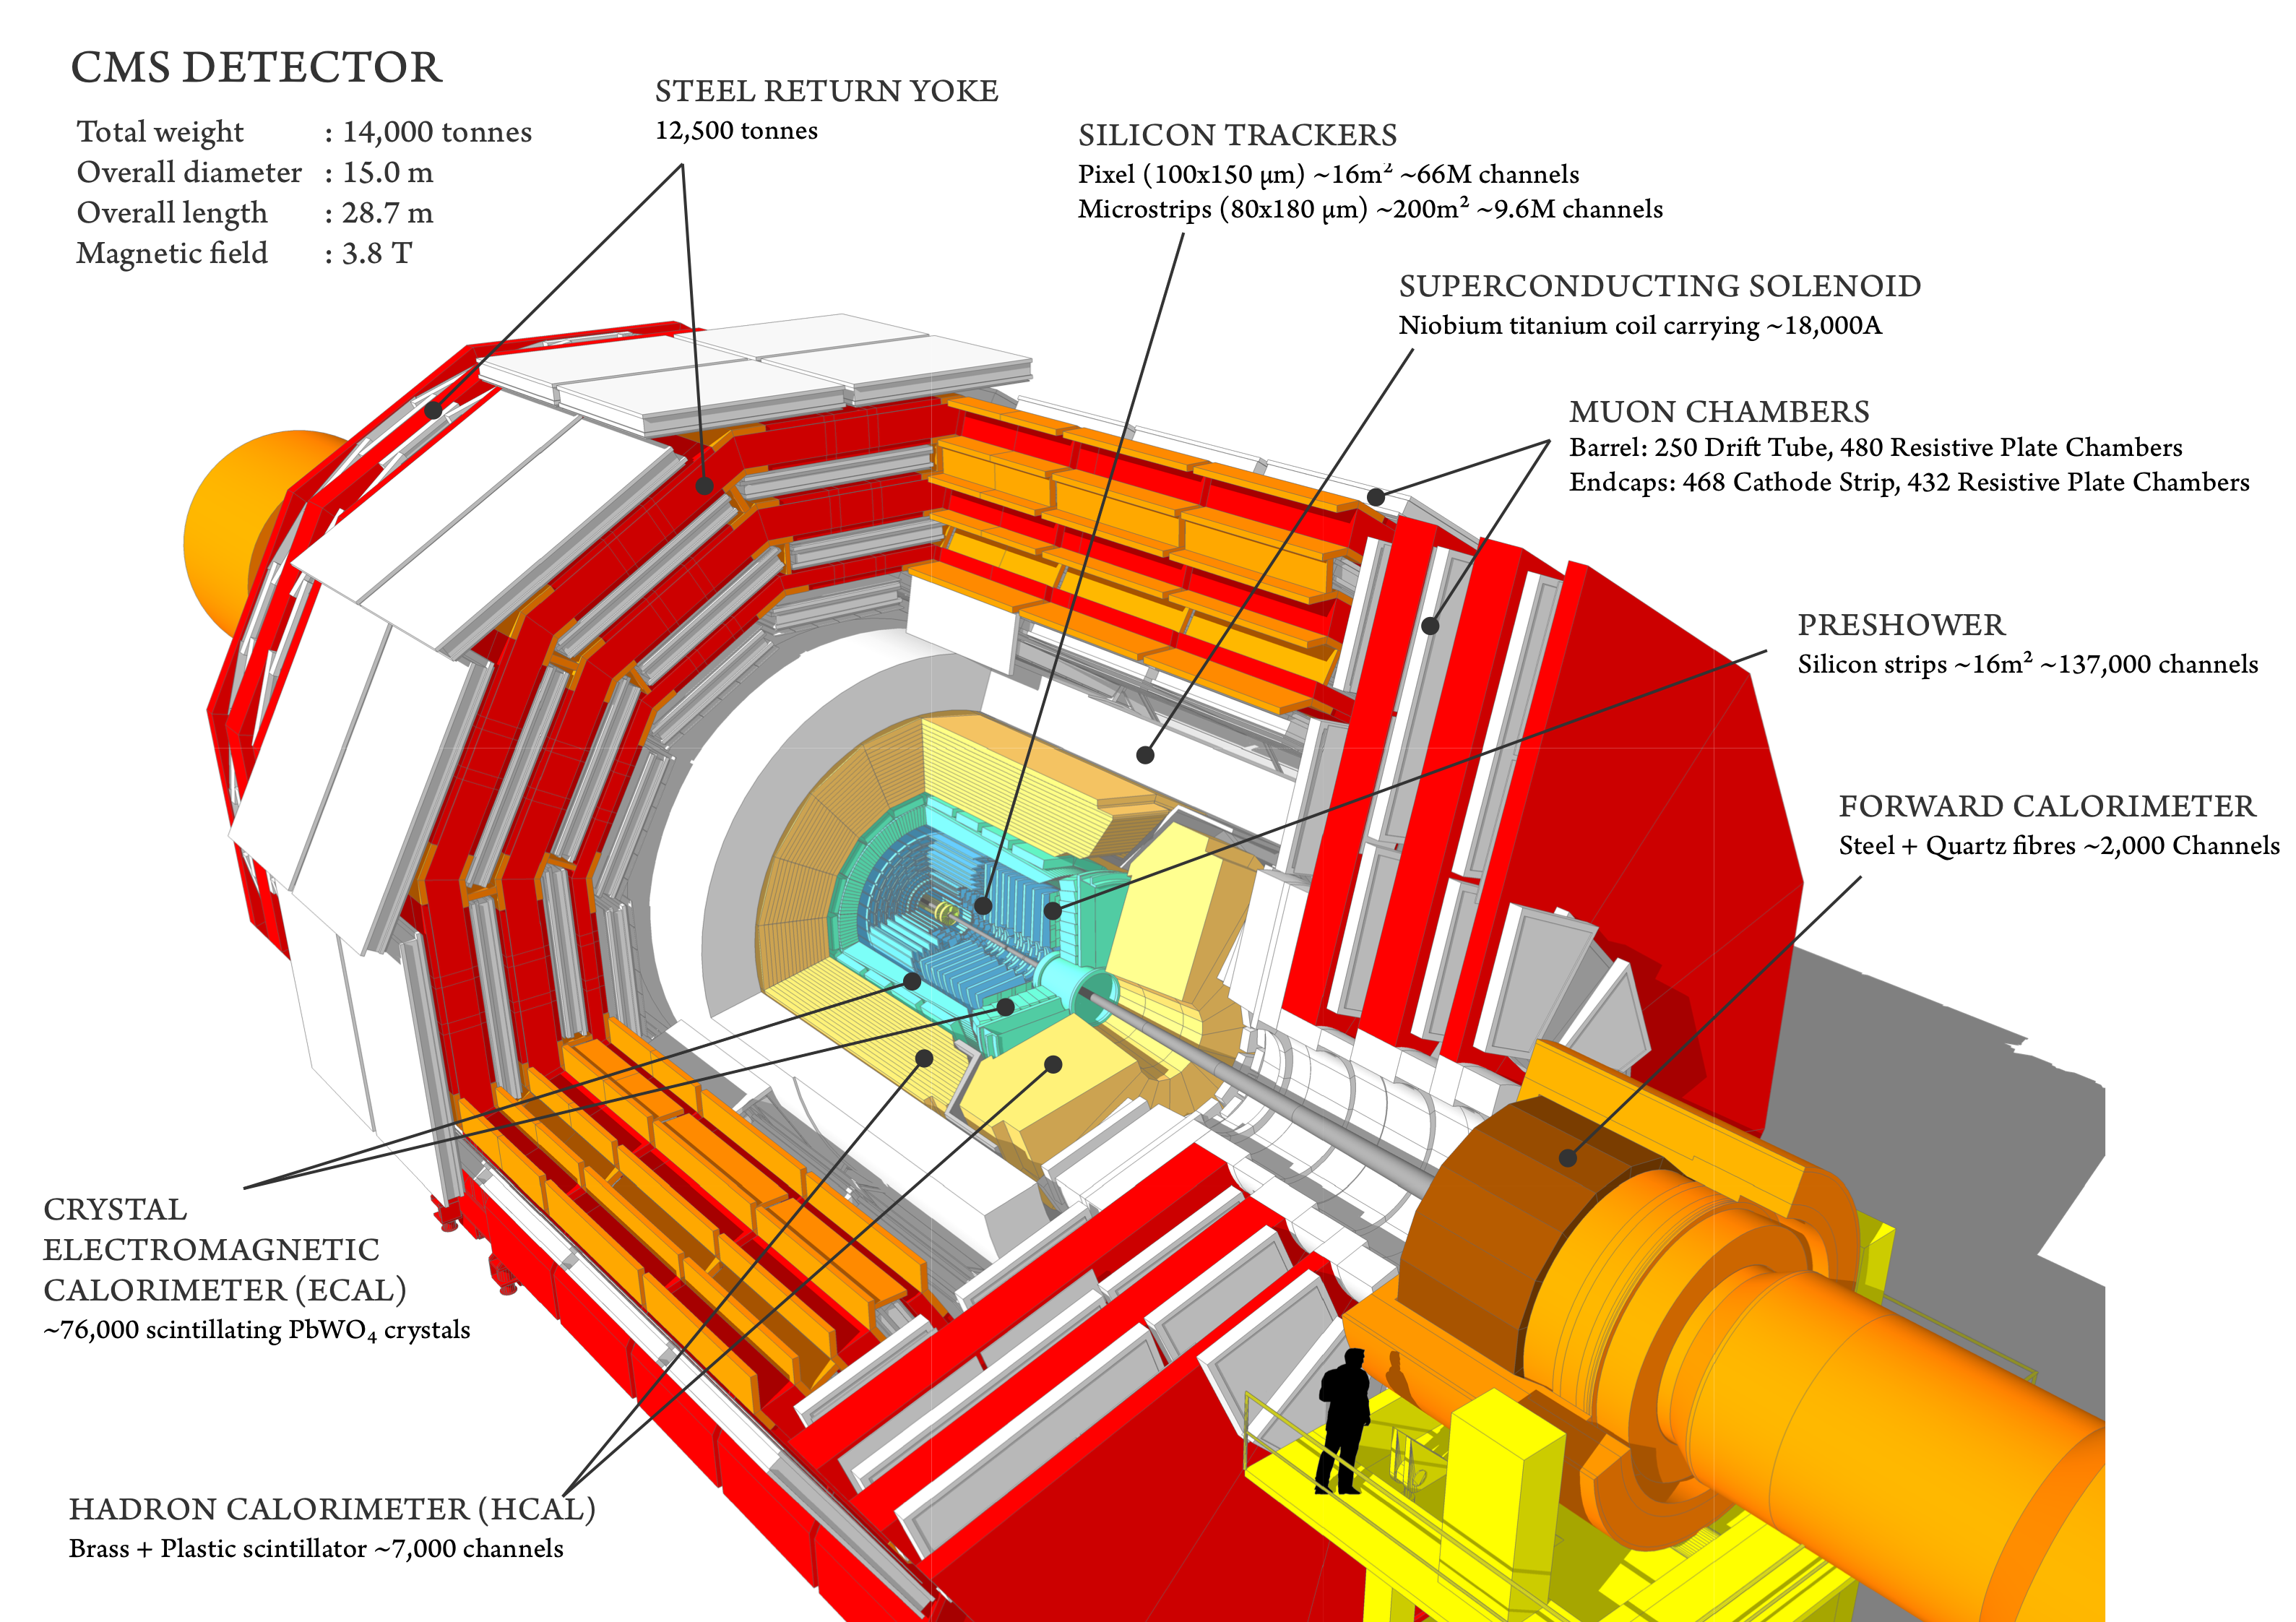
\includegraphics[width=0.8\linewidth]{Figures/chapter2_Figure/CMS_detector_design.png}
\caption{The CMS detector schematic diagram}
\label{Fig:CMS_detector_design}
\end{center}
\end{figure}
\subsubsection{The CMS magnet}
Measuring the momentum of the charged particle with great precision is one the ultimate goals of the CMS detector. In this regards, choice of magnetic field configuration is very important feature of a particle detector like CMS. Stronger magnetic field is needed to measure high energy charged particle momentum with precision. In CMS, this is achieved by selecting the superconducting solenoid magnet. \par
When a charged particle moves in uniform magnetic field of a solenoid, its momentum resolution which depends upon strength of magnetic field and the radius of solenoid, can be written as:
\begin{equation}
	\frac{dp}{p} \propto \frac{p}{Br^{2}} %y = \ln(\frac{E+p_{z}}{E-p_{z}})
\end{equation}

Here $r$ is the path length traversed by the charged particle inside the magnetic field (it becomes radius of the magnetic if the particle passed the full magnet).
It is obvious from the relation, that for detector to obtain high momentum resolution, we need a volumetric solenoid magnet with stronger magnetic field.
CMS solenoid magnet is designed to have bore of diameter 6 m and length 12.5 m producing magnetic field of 3.8 T which is 100,000 time stronger than earth magnet.  It is the largest ever built magnet weighs about 12,000 tonnes. It is powerful enough in providing a strong magnetic field in its dimensions throughout the detector. It surrounds CMS ITS, ECAL and HCAL. 
The strong magnetic field efficiently bends the charged particles when they move through it. More the momentum of the charged particles less they bend, so high energetic charged particles require a stronger magnetic field for its momentum to be measured accurately. CMS aims to have excellent momentum resolution with such  strong magnetic field specially for muons. The schematic diagram of CMS magnet is given in the Figure \ref{Fig:cms_magnet}.
\begin{figure}
\begin{center}
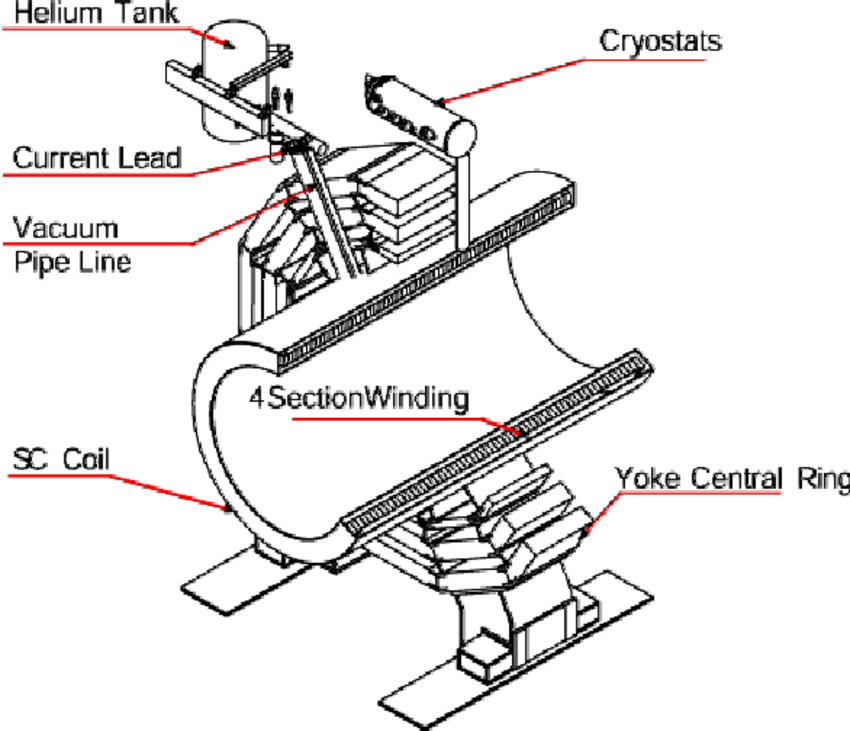
\includegraphics[width=0.45\linewidth]{Figures/chapter2_Figure/magnet_diagram.png} 
\caption{CMS magnet system.}
\label{Fig:cms_magnet}
\end{center}
\end{figure}

The CMS magnetic is made of coil of NbTi wire which becomes a source of uniform magnetic field when current passes through it. The NbTi becomes superconductor at $-268.5^{\circ}$~C (4~K) which allows a huge amount of current (10,000~A) to pass through it. To maintain
this temperature liquid helium is used. 
%A large bending is achieved in tacker by stronger magnetic field providing precise and efficiencies momentum measurement. 
The magnetic field direction inside (tracker) and outside the solenoid (muon system) allows to make second momentum measurement for muons ~\cite{cms:MFTDR,Reference36,Reference37,Reference38}.

%\subsection{CMS Detector Geometry}
\subsection{CMS Coordinate system}
Coordinate system used for CMS detector for its operations is sketched in Figures \ref{fig:cms_coordinates1:a} \ref{fig:cms_coordinates2:a}. %This will be used throughout. 
The CMS detector is in cylinderical shape around beam axis as illustrated in Figure \ref{Fig:CMS_detector_design} which is represented by $Z-axis$ in Figures \ref{fig:cms_coordinates1:a} \ref{fig:cms_coordinates1:a}. The point where two beams collides in beam pipe is called center of experiment; the y axis is directed 
vertically upwards and the x axis being horizontal towards the LHC ring center. 
\begin{figure}[htb]
  \begin{center}
    \subfigure[]{
      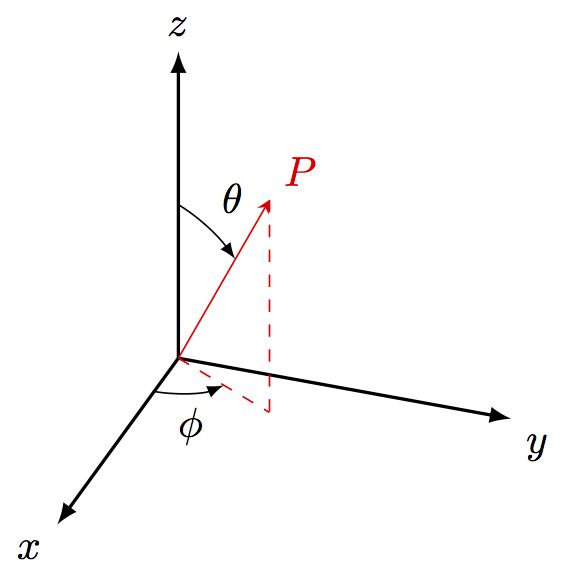
\includegraphics[width=0.30\textwidth,angle=0]{Figures/chapter2_Figure/cms_coordinate_system1.png}
       \label{fig:cms_coordinates1:a}
    }   
    \subfigure[]{
      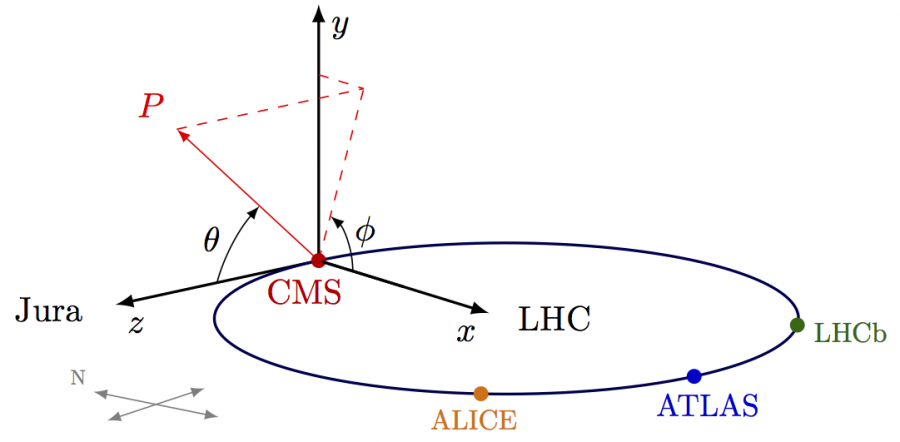
\includegraphics[width=0.65\textwidth,angle=0]{Figures/chapter2_Figure/cms_coordinate_system2.png}
       \label{fig:cms_coordinates2:b}
    } \\
    
          \caption{CMS spherical coordinte system}
  \label{fig:cms_coordinates2:b}
  \end{center}
\end{figure}




%\begin{figure}
%\begin{center}
%
\includegraphics[width=0.8\linewidth]{Figures/chapter2_Figure/CMS_coorinidates.pdf}
%\caption{The CMS Experiment coordinate system.}
%\label{Fig:CMS_coordinates}
%\end{center}
%\end{figure}
The $r$ represents the radial component in transverse plane while $\phi$ is the the azimuthal angle measured from the x axis. 
$\theta$ which is measured from z axis is called polar angle.
%which is measured from the z axis as shown in Figure \ref{Fig:CMS_coordinates}. 
Position of particle when it passes through the CMS is described in terms of $(\eta,\phi)$, where $\eta$ being the pseudo-rapidity defined as  $\eta = -\ln \tan(\theta/2)$ and remains invariant under the longitudinal boosts in the environment of the partons which carry the fractions of the momentum from hard scattering collisions of e.g. proton-proton. 
%As a results, events in CMS detector will have boosted center-of-mass as compared to lab frame along z axis. New defined quantity pseudorapidity  is invariant under 
%these boosts. 
%In short, pseudorapidity is approximation of rapidity in case of high energetic particles which are assumed to be massless and is defined below
%\begin{equation}
% y = \ln(\frac{E+p_{z}}{E-p_{z}})
%\end{equation}
%\begin{equation}
% \approx \ln(\frac{1+\cos\theta}{1-\cos\theta)}
%\end{equation}
%\begin{equation}
% = \ln(\cot^{2}\theta).
%\end{equation}
Moreover, pseudorapidity also helps to differentiate the barrel regions from the endcap regions of sub detectors. In terms of pseudorapidity, the barrel region are defined by 
$|\eta| < 1.5 $ whereas the endcap region corresponds to $1.5 < |\eta| < 3.0$. 
%Formally, electromagnetic calorimeter and tracking system provides a coverage a region up to  $|\eta| < 2.5 $,
% while muon station covers up to $|\eta| < 2.4 $. So, in CMS muons and electrons are selected with $|\eta| < 2.4 $ and $|\eta| < 2.5 $ respectively. As there 
% is no transverse momentum (along y axis) before collisions which leads to have transverse momentum approximately zero.  The transverse energy of any particle 
% is orthogonal to z axis, defined as $E_{T} =  E \sin\theta$ and similarly the transverse momentum $p_T = p \sin\theta$. For a massless particle approximation, 
% electrons and muons, transverse momentum is equal to  transverse energy i.e. $E_T = p_T$.
% \\ As the CMS is hermetic, the energy of those particle which escaped from detector is understood as missing transverse energy. These particles
% can be new physics particles, neutrinos and neutralinos which have no or very little interaction with detector material.
\subsection{Inner Tracking System (ITS) }
 The CMS ITS is a sub-detecting system of the CMS detector which is important form its task to give best tracks  and hence the momenta (above 1~GeV) of the particles (electron, muon, hadrons-quark-structured particles and other short-lived particles) produced in the collisions that take place at CMS, LHC. It is the most inner sub-detector placed under influence of a strong and uniform magnetic field of CMS solenoid and it surrounds the region of beam pipe as shown in Figure \ref{Fig:CMS_detector_design}. 
 ITS also provides the position information of the primary and secondary vertices which is important to reject extra interactions and objects. 
% to be continued

Being in cyliderical shape, it as diameter of about 2.5 m and length about 5.5 m providing $|\eta|$ coverage up to 2.5.  
%The purpose of inner tracking system is to determine the trajectories of the charged particles needed to calculate their momentum and to reconstruct the secondary vertices. The whole ITS is placed in CMS solenoid under influence of a uniform magnetic field of strength 3.8 T. 
At LHC nominal luminosity of $10^{34} cm^2s^{-1}$, there is an average of more than 20 proton-proton interactions (called pileup, for 2018 it was above 30) leading to average about 1000
 particles emerging after every bunch crossing, 25 ns. 
ITS is entirely made up of (200~$m^2$ of) silicon which is benefitted from being super efficienct in the environment of huge flux of particles coming out of the interaction point. 
A schematic diagram of CMS ITS is shown in the figure \ref{Fig:CMS_tracker} (as stood before phase 1 pixel upgrade).

\begin{figure}
\begin{center}

\includegraphics[width=0.8\linewidth]{Figures/chapter2_Figure/CMS_tracker.pdf}
        \caption{Schematic diagram of CMS tracker system. Lines represent detector modules (before phase 1 pixel upgrades ).}
\label{Fig:CMS_tracker}
\end{center}
\end{figure}

%To distinguish the trajectories and assign correct bunch crossing, fast response and high granularity
% detector technology is needed. To protect against radiation damage caused by intense particle 
% flux and priority to minimize the material to avoid from multiple scattering, nuclear reaction, bremsstrahlung and photon conversion, a compromise was 
% found to choose silicon detector technology. 
%CMS inner tracker is made of about 200~$m^2$ of silicon hence being the largest tracker of its kind ever made. 
% \par CMS tracker detector should be robust  which can reconstruct tracks of charged particle in whole pseudorapidity range with momentum above 1~GeV to
% achieve LHC physics goals. Tracker also helps
% to identify other particles like electron, muons along with electromagnetic calorimeter.
% CMS inner operates under intense particle flux with hit
% density varies  from  1~MHz/mm${}^2$ at radial distance of 4cm decreasing to 60~KHz/mm${}^2$ and to 3~KHz/mm${}^2$ at distance of 115cm. 
% Keeping in view of hit densities, different types of detectors are installed at various radial distances of inner tracker listed in Table \ref{Tab:cms_detector_regions}. 
% Silicon detectors are chosen
% due its unique properties of fast response and good spatial resolution which enables it to work efficiently even in high radiation environment. 
To limit the damage mainly by  radiation ITS is kept at about -20$^{\circ}$ C. Full ITS is an assembly of a pixel detector and silicon strip tracker.
%\begin{table}
%\begin{center}
%\caption{Types of detectors installed in CMS tracking system.}
%\label{Tab:cms_detector_regions}
%\begin{tabular}{cccc}
%  \hline
%Section & Radial distance (cm) & Detector type & Cell size \\
%\hline
%Pixel   & $r<10$ & pixel & $100\mu m~\times150\mu m$ \\
%TIB+TID & $20<r<55$ & microstrips & $10cm~\times150\mu m$\\
%TOB+TEC & $55<r<110$ & strips & up to $25cm~\times180\mu m$\\
%\hline
%\end{tabular}
%\end{center}
%\end{table}
% %\par The CMS inner tracker schematic drawing is shown in Figure~\ref{Fig:CMS_tracker}~\cite{Reference34}. Tracker most inner region is the pixel detector that is nearest to the 
\subsubsection{The Pixel Detector}
Part of the tracker system which is nearest to the interaction point is the Pixel detector.
%The CMS inner tracker schematic drawing (as it stood before phase 1 upgrades) is shown in Figure ~\ref{Fig:CMS_tracker} ~\cite{Reference34}. 
%Tracker most inner region is the pixel detector that is nearest to the 
% interaction point consists of disk modules on each side and barrel layers. 
%It provides accurate traces in $z$ and $r-\phi$ with a pixel cell of  size $100\times150\mu m^2$ covering the $|\eta|$ range up to 2.5. Pixel detector also plays its role for impact parameter resolution that helps to
Silicon modules of the pixel detector, are facilitated with pixel cells of  size $100\times150\mu m^2$ each providing the $|\eta|$ range up to 2.5. 
It helps to reconstruct the secondary vertex and delivers three spatial points precisely throughout its geometry ~\cite{Reference34}. %  with the Pixel detector also plays its role for impact parameter resolution that helps to
% reconstruct secondary vertex ~\cite{Reference34}.
% Pixel detector delivers three spatial point with excellent precision throughout the coverage of pixel. % \ref{Fig:CMS_pixel}~\cite{Reference34}. 

 \par During data taking of Run 1 operations of LHC, some dynamic inefficiencies (about 5\% at an event pile-up of 40~)  were reported in the first layer of barrel of pixel sub-detector, due to the limited size of the readout
bandwidth. Subsequently, a new pixel detector was installed in March 2017 Ref. \ref{Klein:2017nke}, equipped with one additional barrel  % The Phase-2 Upgrade of the CMS Tracker. Available online: https://cds.cern.ch/record/2272264 (accessed on 7 January 2019)
%@article{Klein:2017nke,
%    author = "Tumasyan, Armen and others",
%    editor = "Klein, K.",
%    collaboration = "CMS",
%    title = "{The Phase-2 Upgrade of the CMS Tracker}",
%    reportNumber = "CERN-LHCC-2017-009, CMS-TDR-014",
%    month = "6",
%    year = "2017"
%}
layer and one additional forward disk. In the new pixel detector, the innermost layer is closer to the
interaction point and the outermost one is further away from it as it is shown in Fig.  \ref{Fig:CMS_pixel_upgrade} %(Figure 1)

\begin{figure}
\begin{center}
%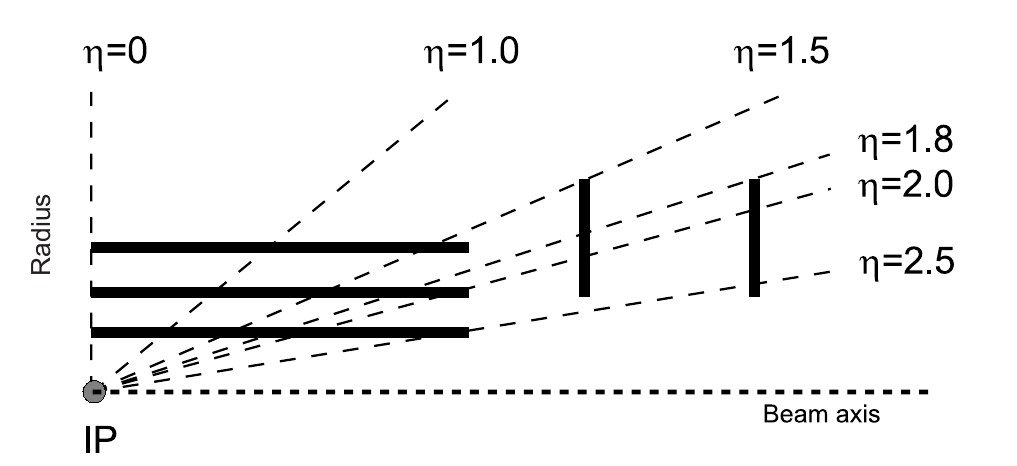
\includegraphics[width=0.8\linewidth]{Figures/chapter2_Figure/rename.png}
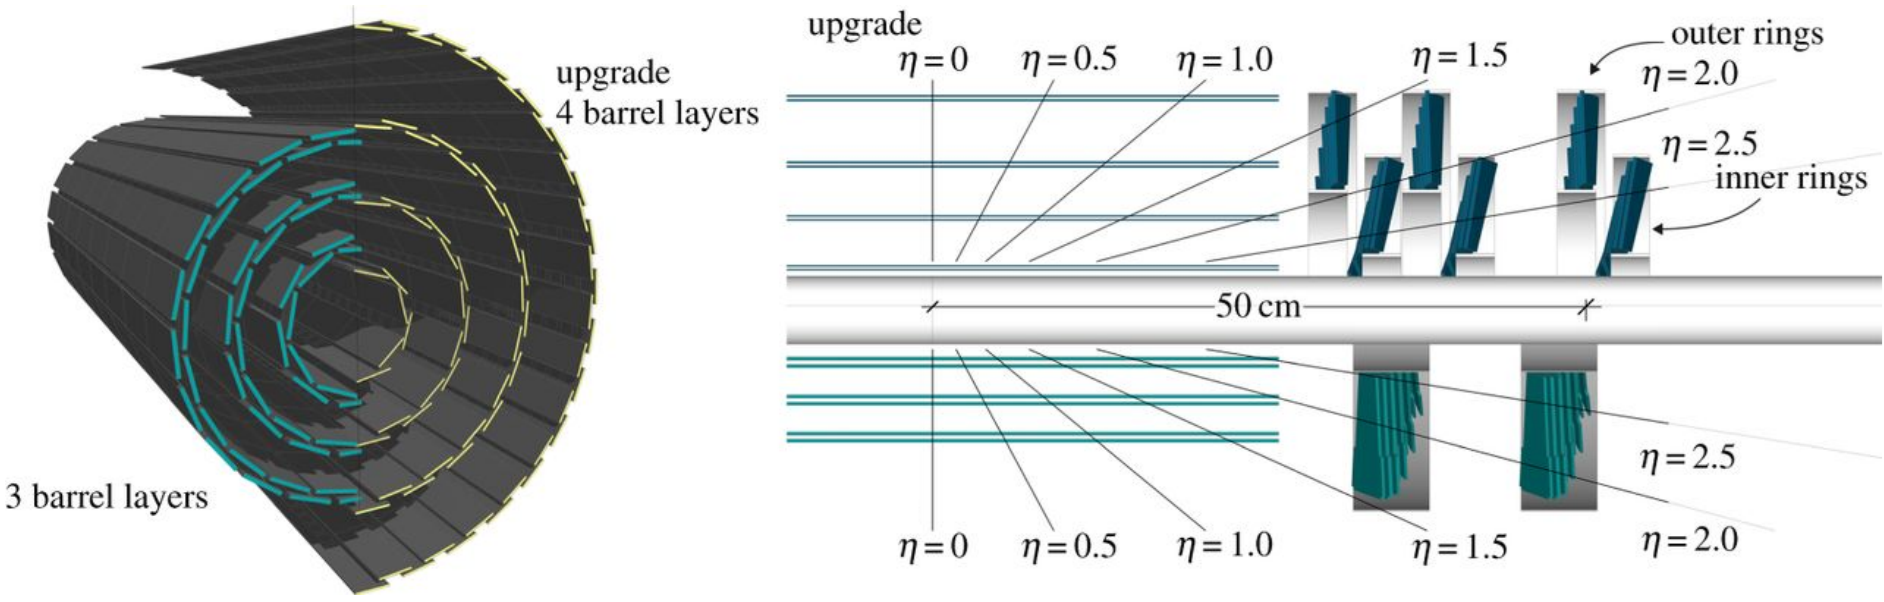
\includegraphics[width=0.8\linewidth]{Figures/chapter2_Figure/CMS_pixel_upgrade.png}
%\caption{CMS pixel detectors and hit coverage. Lines represent detector modules.}
\caption{Schematic diagram of pixel detector's upgrade. Old pixel detector is shown by the lower half detector, and the new pixel detector is represented by the upper half.}
\label{Fig:CMS_pixel_upgrade}
\end{center}
\end{figure}\\

It also uses new Readout Chips (ROCs) benefitted from reduced data loss at higher collision rates with respect to Phase 1 operations (at 160 Mbit/s).
Bandwidth of the readout electronics was increased approximately by a factor of eight
(320 Mbit/s). In addition, DC-DC power converters were installed to allow reusing the existing fibers
and cables. Hence, the upgraded pixel detector has a higher rate capability and number of channels,
providing increased tracking efficiency, reduced fake rate, and improved impact parameter resolution.
In the figure ~\ref{Fig:hit_efficiency_upgrade}, clear improvments in the dynamic efficiency of 2017 (with pixel upgrades) with respect to the 2016 (without pixel upgrades) can be seen Ref. ~\cite{Sonneveld:2018ntf}.

\begin{figure}
\begin{center}
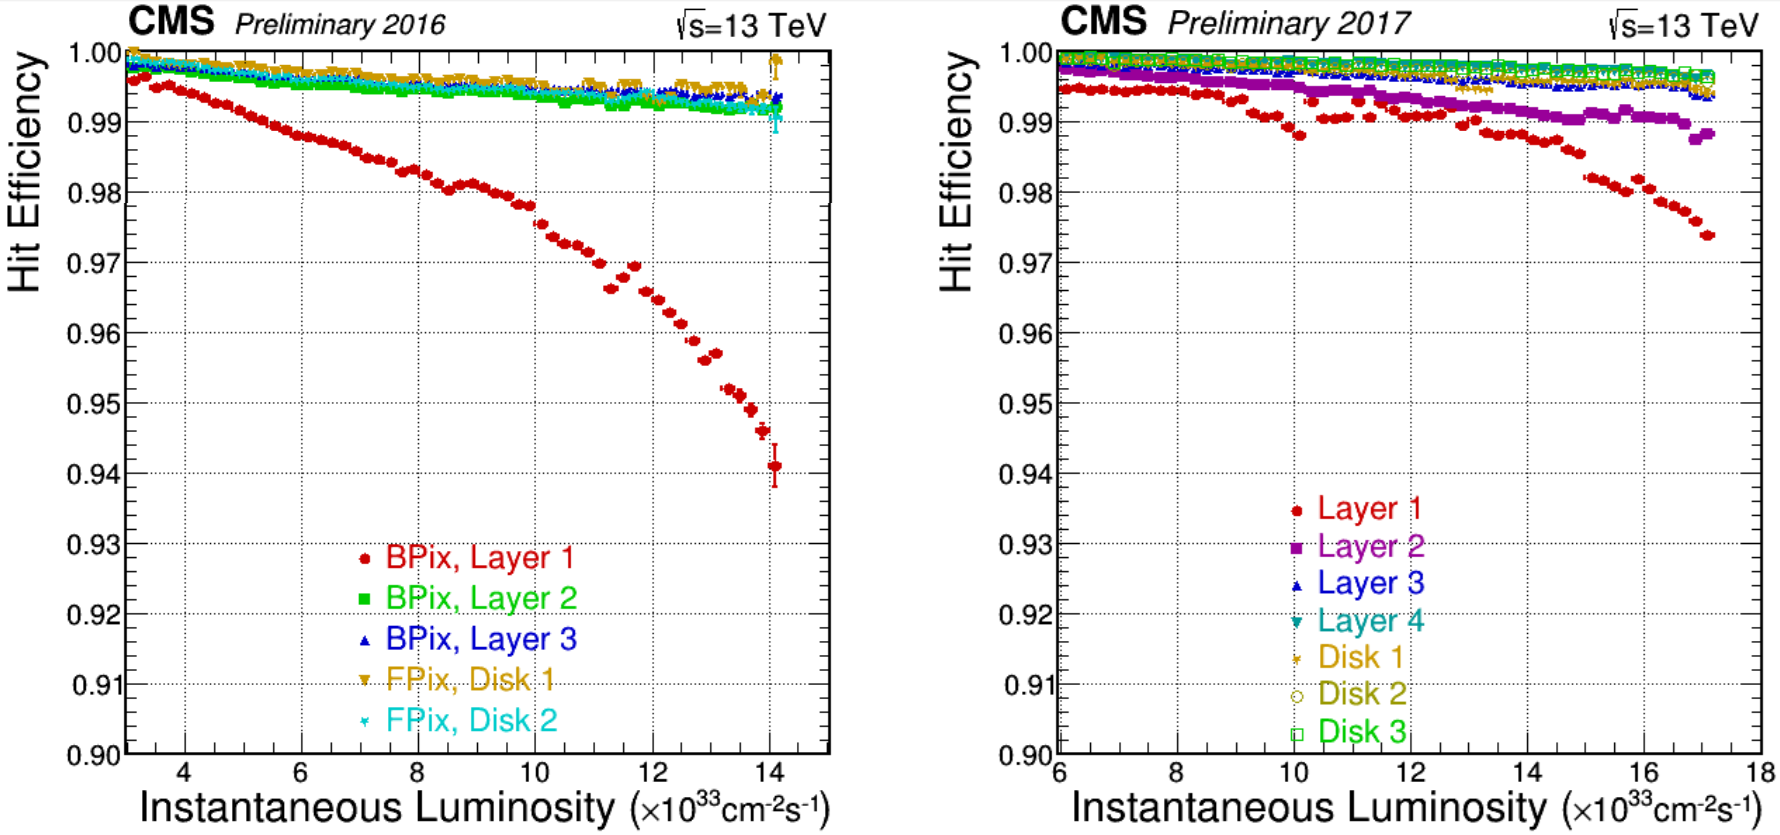
\includegraphics[width=0.8\linewidth]{Figures/chapter2_Figure/hit_efficiency_upgrade.png}
%\caption{CMS pixel detectors and hit coverage. Lines represent detector modules.}
        \caption{Pixel detector's hit efficiency as function of instantaneous luminosity corresponding to 2016 data (left) and to 2017 data (right) } %[in comments] }  % Sonneveld, J. Commissioning and first results from the CMS phase 1 upgrade pixel detector. In Proceedings of the 26th International Workshop on Vertex Detectors, Las Caldas, Asturias, Spain, 10–15 September 2017; PoS(Vertex 2017)018.
\label{Fig:hit_efficiency_upgrade}
\end{center}
\end{figure}

Overall, the pixel detectors is of 1~$m^2$ size containing 66 million pixels.  % to be updated ?? 

\subsubsection{The Silicon Strip}
Next layer to the pixel detector is called Silicon Strip Tracker which is installed at radial distance  from 20cm to 116cm.  
%Silicon Strip is the second layer detector after pixel detector which is installed at  radial distance  from 20cm to 116cm. 
This detector surrounds both sides of pixel with Its tacker inner barrel (TIB, 4 layers) and  tracker inner disk (TID, 3 layers) surrouds the pixel detector and extend upto 20 cm-50 cm where silicon microstrips of thickness $320\mu$m are installed.
Both are surrounded the Tracker outer barrel (TOB, 6 layers) which is 220 cm long and provides z coverage up to 118 cm. 
In barrel and endcap regions, the pitch of strips changes from 80$\mu$m to 120$\mu$m and 100$\mu$m to 141$\mu$m respectively.
%There are 3 disks on each endcap and 4 barrel layers where silicon microstrips of thickness $320\mu$m are installed. 
%Microstrips
% are aligned along with beam axis in the barrel region and in radial direction on disks. The strip pitch in barrel region varies  from 80$\mu$m to 120$\mu$m
% from inner to outer barrel layer. In the endcap region strip pitch changes from 100$\mu$m to 141$\mu$m. 
Finally, the most outer part of CMS tracker system  is tracker outer barrel (TOB) installed at radial distance from 55cm to 116cm containing 500$\mu$m thick 6 barrel layers with strip pitch of 183$\mu$m and 122$\mu$m. 
Beyond z=118 cm, there are tracker endcaps (TEC+, TEC-, 9 discs) which cover 124 cm$<|z|<$282 cm and 22.5 cm$<|r|<113.5$ cm providing coverage of $|\eta|$<2.5.
%As mentioned, in the previous sections, measuring momenta in CMS tracker we exploit the bending properties of magnet

%\begin{figure}
%\begin{center}
%
\includegraphics[width=0.8\linewidth]{Figures/chapter2_Figure/CMS_tracker.pdf}
%	\caption{Schematic diagram of CMS tracker system. Lines represent detector modules (before phase 1 pixel upgrades ).}
%\label{Fig:CMS_tracker}
%\end{center}
%\end{figure}
% \begin{figure}
%\begin{center}
%%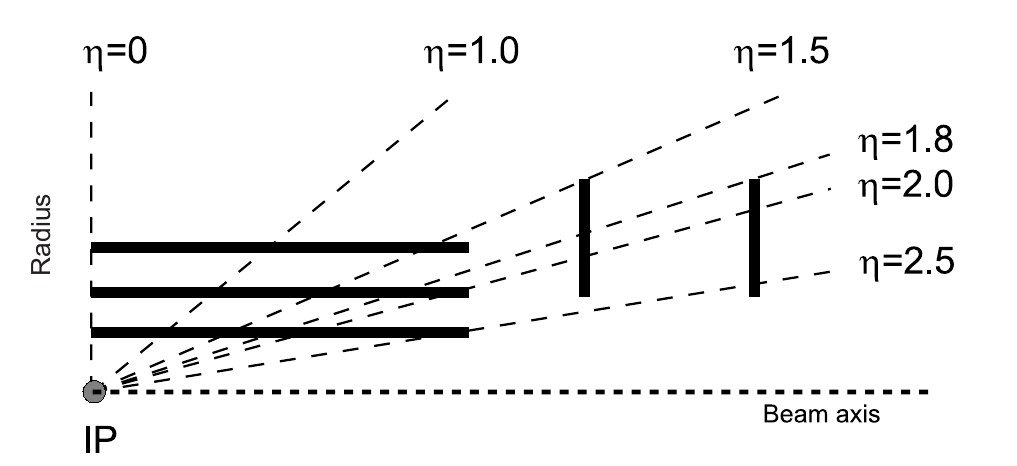
\includegraphics[width=0.8\linewidth]{Figures/chapter2_Figure/rename.png}
%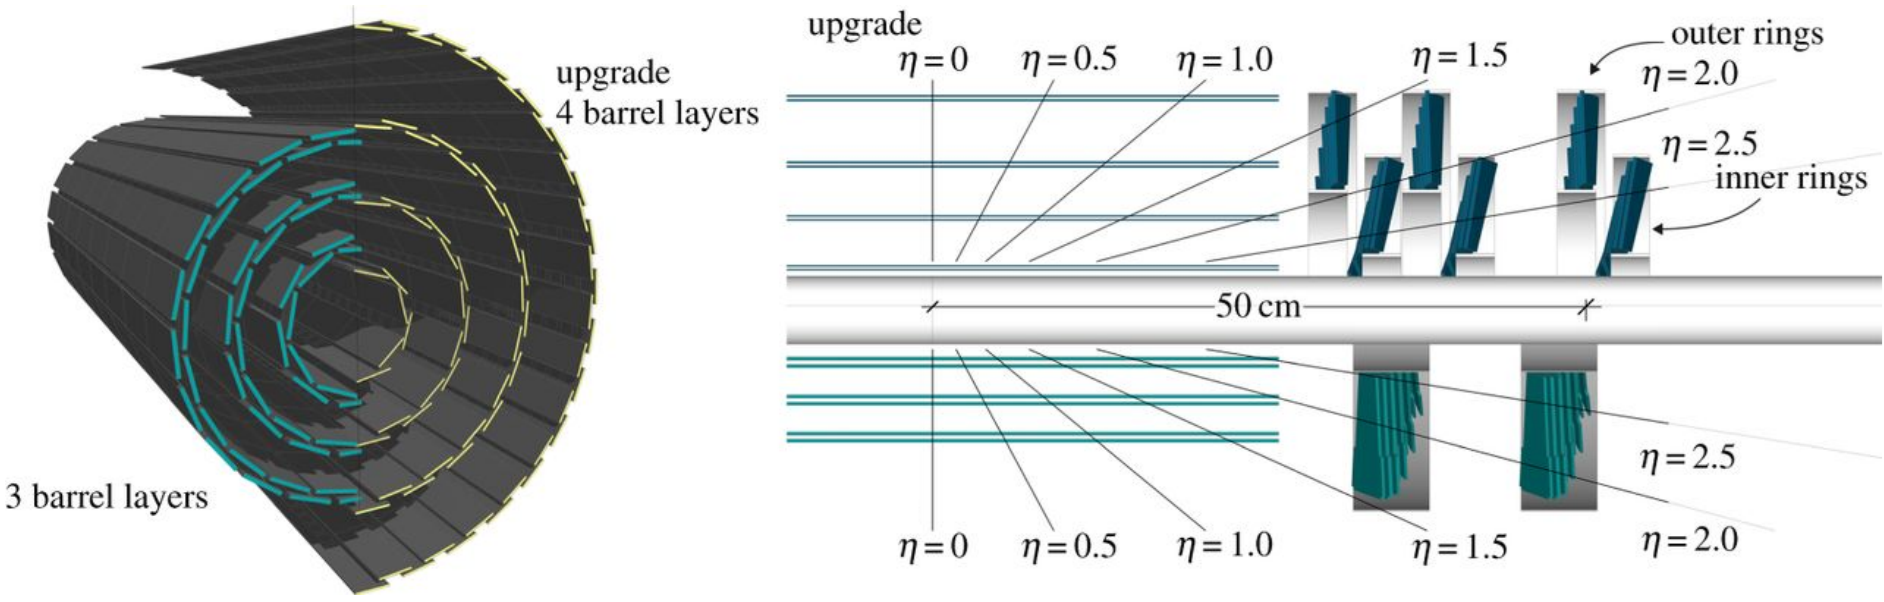
\includegraphics[width=0.8\linewidth]{Figures/chapter2_Figure/CMS_pixel_upgrade.png}
%%\caption{CMS pixel detectors and hit coverage. Lines represent detector modules.}
%\caption{Schematic diagram of pixel detector's upgrade. Old pixel detector is shown by the lower half detector, and the new pixel detector is represented by the upper half.}
%\label{Fig:CMS_pixel_upgrade}
%\end{center}
%\end{figure}\\
%\par To measure the  momentum in CMS tracker, we simply exploit the property of the charged particles to bend in the magnetic field. High momentum particles
%will bend less in detector and vice versa, making resolution worse due to less curvature. 
%\par The upgraded pixel detector improved $\Hllll$ analysis as there was significant increase in lepton number in an event thus improving the reconstruction of Z candidates and hence an increase in the selection efficiency upto much extent. [Ref. CMS-TDR-011]
%\begin{figure}
%\begin{center}
%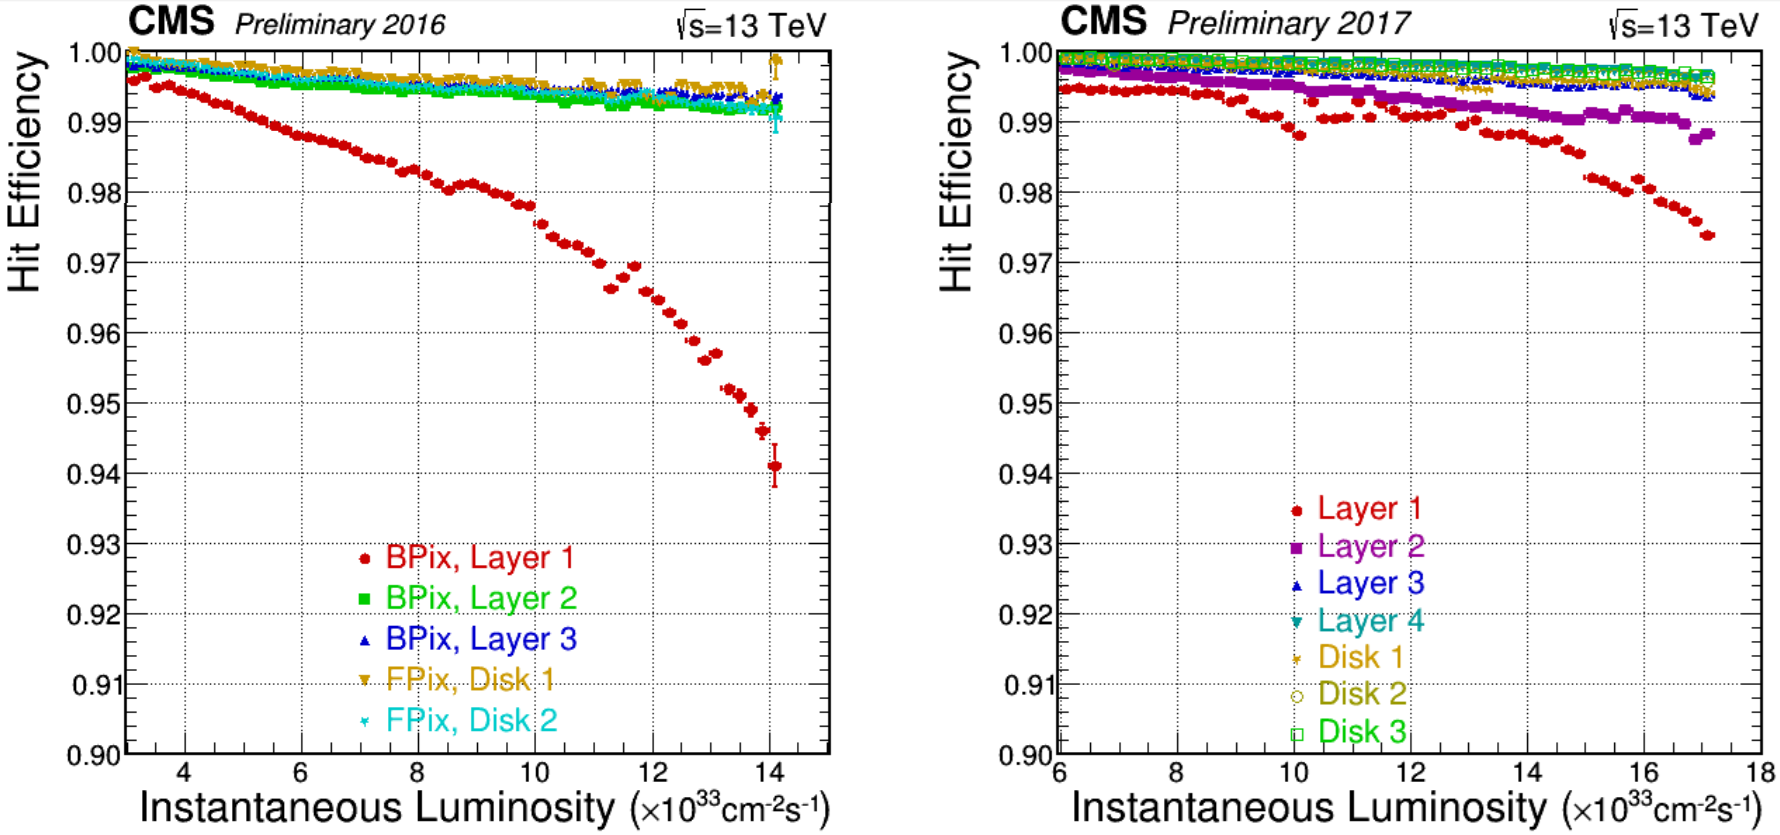
\includegraphics[width=0.8\linewidth]{Figures/chapter2_Figure/hit_efficiency_upgrade.png}
%%\caption{CMS pixel detectors and hit coverage. Lines represent detector modules.}
%	\caption{Pixel detector's hit efficiency as function of instantaneous luminosity corresponding to 2016 data (left) and to 2017 data (right) } %[in comments] }  % Sonneveld, J. Commissioning and first results from the CMS phase 1 upgrade pixel detector. In Proceedings of the 26th International Workshop on Vertex Detectors, Las Caldas, Asturias, Spain, 10–15 September 2017; PoS(Vertex 2017)018.
%\label{Fig:hit_efficiency_upgrade}
%\end{center}
%\end{figure}
%
%%The material in radiation length's for different sub detectors and functional modules are shown in Figure~\ref{Fig:CMS_tracker_material}~\cite{Reference34}. As in tracker, strips and pixel sizes are not uniform with 
%%the variation of $\eta$, Figure~\ref{Fig:CMS_tracker_expected_efficiency}~\cite{Reference34} shows the expected performance of muon tracks resolution with $p_T$= 1, 10 and 100~GeV as function
%% of $|\eta|$. While Figure~\ref{Fig:CMS_tracker_global_efficiency}~\cite{Reference34} shows  comparison of global track reconstruction efficiencies of muons and pions with 
%% same transverse momentum. 
%%\begin{figure}
%%\begin{center}
%%
\includegraphics[width=0.8\linewidth]{Figures/chapter2_Figure/tracker_meterial.pdf}
%%\caption{Material in radiation length's for different sub detectors (left) and for different functional modules (right) as function of $\eta$}.}
%%\label{Fig:CMS_tracker_material}
%%\end{center}
%%\end{figure}
%% \begin{figure}
%%\begin{center}
%%
\includegraphics[width=0.8\linewidth]{Figures/chapter2_Figure/expected_efficiency.pdf}
%%\caption{Expected single muons tracks resolution of transverse momentum (left), transverse impact parameter (middle) and longitudinal impact parameter (right)
%%of $p_T = $ 1, 10, 100 GeV.}
%%\label{Fig:CMS_tracker_expected_efficiency}
%%\end{center}
%%\end{figure}
%%\begin{figure}
%%\begin{center}
%%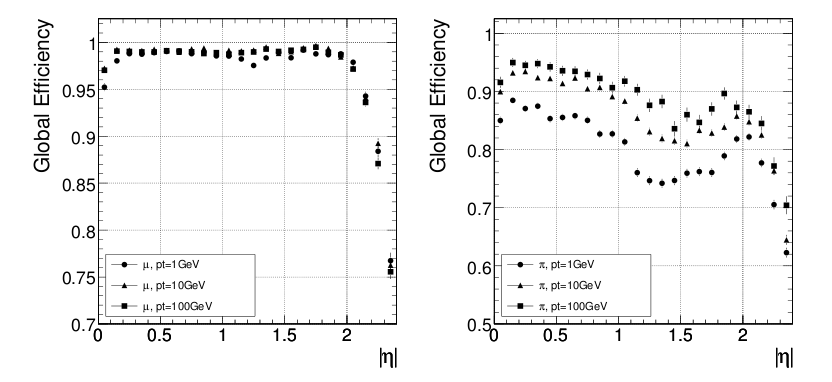
\includegraphics[width=0.8\linewidth]{Figures/chapter2_Figure/global_efficiency.png}
%%\caption{CMS tracker global efficiency of muons (left) and pions (right) of $p_T = $ 1,10, 100 GeV.}
%%\label{Fig:CMS_tracker_global_efficiency}
%%\end{center}
%%\end{figure}

\subsection{Electromagnetic Calorimeter (ECAL) }
ECAL is the cylindrical shaped homogeneous calorimeter built with 75848 crystals of lead tungstate (PbWO${}_4$) placed inside the CMS solenoid magnet. Its barrel ergion (EB) contains 61200 PbWO${}_4$ crystals and provides pseudorapidity coverage of $|\eta| < 1.479$. Endcap region of the ECAL
(EE) is built with 7324 crystals on either side in endcap regions and provides pseudorapidity coverage up to $\eta < 3$. 
The region of $1.4442 < |\eta| <1.56$ is regarded as crack region between barrel and endcaps as can been seen in Figure \ref{Fig:CMS_ECAL_rapidity_cov} taken from ~\cite{Reference34}. This region is excluded for  physics analysis.\\
When high energy particle (e.g. electron or photon) coming out of the collision point enters ECAL, it produces bunch or cascade of particles (electron through bremsstrahlung and photon through pair production) with relatively lower energies. This is called EM showering that continues until electrons dominate in ionization and photon energy becomes less than pair-production threshold. \\
Photodetectors Avalanche photodiodes (APDs) in barrel region and the Vacuum phototriodes (VPTs) in endcap regions are installed which efficiently work under high magnetic field environment ~\cite{cms:ECALTDR}. Response of ECAL comes with emission of light that is directly proportional incident particle's energy (through ionization).

%Higgs discovery (both in $H\rightarrow \gamma\gamma$ and $H \rightarrow ZZ \rightarrow 4\ell$ channels) is based on one of the ECAL key feature in the  design is to reconstruct
A preshower detector is installed in endcap regions to distinguish between single photon and closeby diphoton candidate e.g neutral pion decay ($\pi^{\circ} \rightarrow \gamma\gamma $). Providing pseudorapidity coverage of $1.653<|\eta|<2.6$, it helps to efficiently determin the position of an electron and a photon.

\begin{figure}
\begin{center}
%
\includegraphics[width=0.7\linewidth]{Figures/chapter2_Figure/CMS_Electromagnetic_calorimeter.pdf}

\includegraphics[width=0.7\linewidth]{Figures/chapter2_Figure/ecal_2.pdf}
\caption{CMS ECAL pseudo-rapidity coverage.}
\label{Fig:CMS_ECAL_rapidity_cov}
\end{center}
\end{figure}
%Specially designed Avalanche photodiodes (APDs) and the Vacuum phototriodes (VPTs) are employed in barrel and endcaps region respectively ensure efficient working under high magnetic field. Higgs discovery (both in $H\rightarrow \gamma\gamma$ and $H \rightarrow ZZ \rightarrow 4\ell$ channels) is based on one of the ECAL key feature in the  design is to reconstruct
%electrons and photons with high resolution. 
%%enabled us to discover Higgs boson in both $H\rightarrow \gamma\gamma$ and $H \rightarrow ZZ \rightarrow 4\ell$ favorable channels. 
Lead tungstate is benefitted as it helps to make ECAL compact with high granularity due to the fact that it is denser (8.28 g/cm${}^{3}$) with less radiation length (X_$\circ$ of 0.89~cm ). 
Also, lead tungstate has small Moli\`{e}re radius, which defines the area of deposited energy, helping to minimize the effect of pileup while measuring the energy.
Other important factor is that crystals of lead tungstate have decay time of scintillation about 25 ns which is also the time of LHC bunch crossing.\\
ECAL operating temparature is around 18${}^{\circ}$C and light emitted from the scintillation process is temperature dependent. So, in order to maintain the temperature at nominal value, cooling system is installed which is based on water circulation through Aluminium pipes and is capable enough to maintain the temperature of detector upto $18\pm0.05^{\circ}$ C. Layout of the ECAL of CMS detector is shown in the Figure. \ref{Fig:CMS_ECAL_layout}.

%\subsubsection{ECAL Crystals and Geometry}
%To make a compact and high granularity calorimeter which could fit inside the CMS solenoid, lead tungstate was the best option which is denser than
%steel (8.28 g/cm${}^{3}$) with short radiation length (X_$\circ$) of 0.89~cm~\cite{cms:ECALTDR}. The scintillator (PbWO${}_4$) emits light which is directly proportional to incident particle's energy through ionization. Fast response  (same order of LHC bunch cross crossing i.e. 25ns) of PbWO${}_4$ makes it ideal for 
%ECAL. 
%In barrel region, there are 8.14 m${}^3$ active crystals  installed weighting up to 67.4 tonne. The each crystals cross section is measured to be 
%22~$\times$~22 mm${}^{2}$ in barrel and 28.62~$\times$~28.62 mm${}^{2}$ at endcaps. 
%Crystal length in barrel and endcaps is 230mm and 220 mm which is 25.8 and 24.7 times of the radiation length. 
%\par The amount of emitted light from scintillator and amplification of photodiodes both are temperature dependent. The nominal temperature at which ECAL operates is around 18${}^{\circ}$C. 
%For this reason, cooling system has been installed in ECAL to maintain the temperature at nominal value. The cooling system rotates water at
%18${}^{\circ}$C through parallel grid of aluminium pipes a to maintain the temperature in the detector. In the barrel region, each supermodule has its independent
%supply of water. The cooling system of  the ECAL work efficiently  and maintain the temperature of $18\pm0.05^{\circ} C$.
%
%\begin{table}[!htpb]
%\caption{ECAL crystal details at endcaps and barrel regions.}
%\label{Tab:ecal_crystal_barrel_endcap}
%\begin{tabular}{lll}
%                   & Barrel & Endcaps \\
%\hline
%                   Number of crystals & 61200 & 14648 \\
% Crystal cross section in ($\eta,\phi$) & $0.0174 \times 0.0174$ & variable \\
% Cross section of front face of crystal & $22 \times 22 mm^2$ & $28.62 \times 28.62 mm^2$ \\
% Cross section of rear face of crystal & $26 \times 26 mm^2$ & $30 \times 30 mm^2$ \\
% Crystal length 		       & 230 mm & 220 mm \\
% Crystal length(in terms of $X_{\circ}$) & 25.8$X_{\circ}$ & 24.7$X_{\circ}$ \\
% \hline
% 
%\end{tabular}
%\end{table}
%
\begin{figure}
\begin{center}

\includegraphics[width=0.7\linewidth]{Figures/chapter2_Figure/CMS_Electromagnetic_calorimeter.pdf}
%
\includegraphics[width=0.7\linewidth]{Figures/chapter2_Figure/ecal_2.pdf}
\caption{CMS ECAL layout }
\label{Fig:CMS_ECAL_layout}
\end{center}
\end{figure}
%
%\subsubsection{Photodetectors}
%The requirements on photodetectors are to be fast, robust and able to work efficiently in a region that contains 3.8 T magnetic field. Considering these requirements, different types
%of photodetectors are installed both in the barrel and the endcap regions. In the barrel region, each crystal a pair of avalanche photodiodes are mounted with of 5~$\times$~5~mm$^{}^{2}$ active area. Gain of the working APD is 50 and in parallel read out. 
%%page 35 ?
%In endcap region, a specially designed vacuum phototriodes at National Research 
%Institute Electron(St. Petersburg) for CMS ECAL was used. These are single gain photomultipliers with mean gain being 10.2~ in absence of field. The diameter of each VPT is 22mm.  The total
%active area is almost 280mm${}^2$ where one VPT is attached at the back of every crystal. Their fine coper anode makes them capable to work under 
%intense magnetic field. As compared to APDs, VPTs have lower quantum efficiency and the internal gain which is balanced out with the larger
%back face crystal coverage. The summary of number of the crystals with their dimensions are summarized in Table \ref{Tab:ecal_crystal_barrel_endcap}.
%\subsubsection{Preshower}
%\par Purpose of the installation of preshower detector is the identification of neutral pions detected in the endcaps regions. Due to its high granularity, the preshower helps to differentiate between electron and minimum ionizing particles (MIPs) and to determine the position of electrons and photon. It provides the pseudorapidity coverage of $1.653<|\eta|<2.6$. 
%\subsubsection{Energy Resolution}

Energy resolution of ECAL, which is the ability of detecting system to accurately measure energy of incident radiation, can be written as  
\begin{equation}
	\left(\frac{\sigma}{E}\right)^{2}= \left(\frac{A}{\sqrt{E}}\right)^{2}+\left(\frac{\sigma_{n}}{E}\right)^2+c^2
\end{equation}
where $A$ is stochastic term (defines the intrinsic statistical fluctuations in shower,  in energy deposits of preshower, and the photo(electron)-statistics contributions),  $\sigma_{n}$ is the electronics noise term and $c$ is constant that covers the constant factors such as non-uniformity in detector for light collection and etc.  
Contribution of each term to the energy resolution is shown in the Figure. ~\ref{Fig:ecal_contributions}.
\begin{figure}
\begin{center}
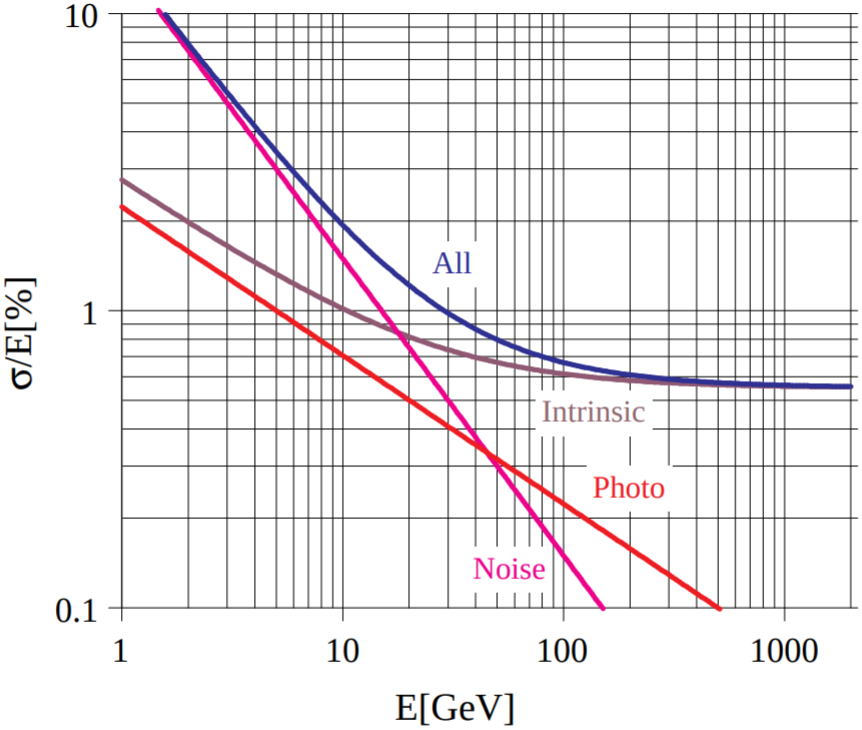
\includegraphics[width=0.60\linewidth]{Figures/chapter2_Figure/ecal_contributions.png}
\caption{CMS ECAL energy resolution curve with individual term contributions.}
\label{Fig:ecal_contributions}
\end{center}
\end{figure}


%term xtracted by fitting the measured points to the function, N being noise term and S is stochastic term. 
%%A measurement of energy resolution has been made by using electron of energies from 20 to 250~GeV in test beam~\cite{Reference35}. The measurement was made by considering arrays of $3\times 3$ or $5 \times 5$. No correlated significant noise was observed in these arrays. The measurements summary is shown in 
A recent study on relative energy resolution of ECAL using 2017 data and MC has been performed using Z events decaying to a pair of electrons. The resolution plots for bremsstrahlung electrons ($R_{9}$>0.94 and $R_{9}$<0.94) is separately shown for data and MC in the Figure \ref{Fig:CMS_ECAL_energy_resolution} ~\cite{Zghiche_2019}.  % https://iopscience.iop.org/article/10.1088/1742-6596/1162/1/012001/pdf 
For $\Hllll$ analyses, excellent energy resolution for leptons is important for precise measurements for which ECAL of CMS plays an important role as it did for Higgs discovery.
\begin{figure}
\begin{center}
%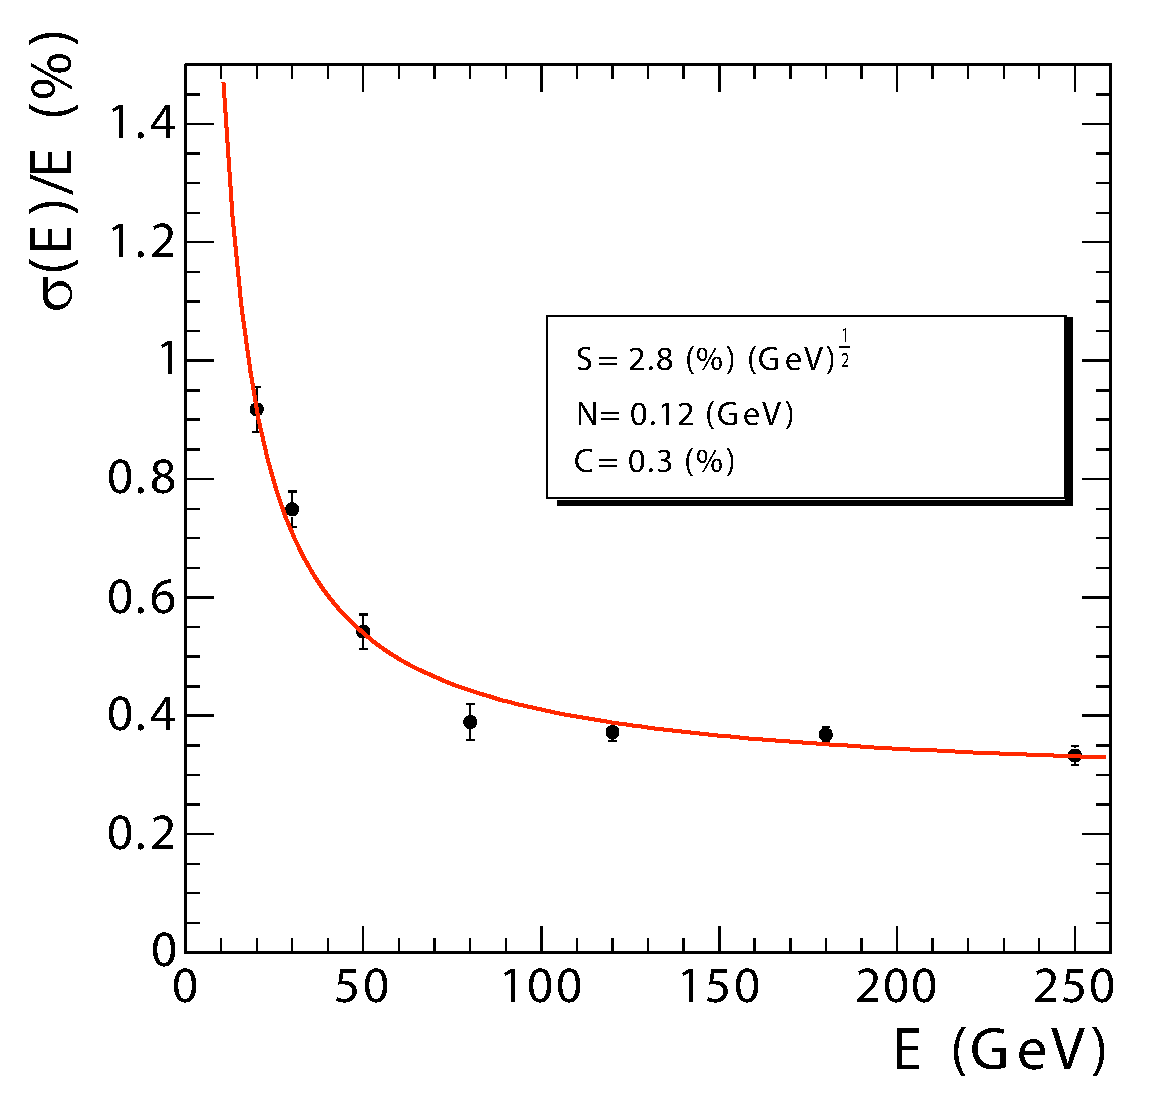
\includegraphics[width=0.7\linewidth]{Figures/chapter2_Figure/ecal_energy_resolution.pdf}
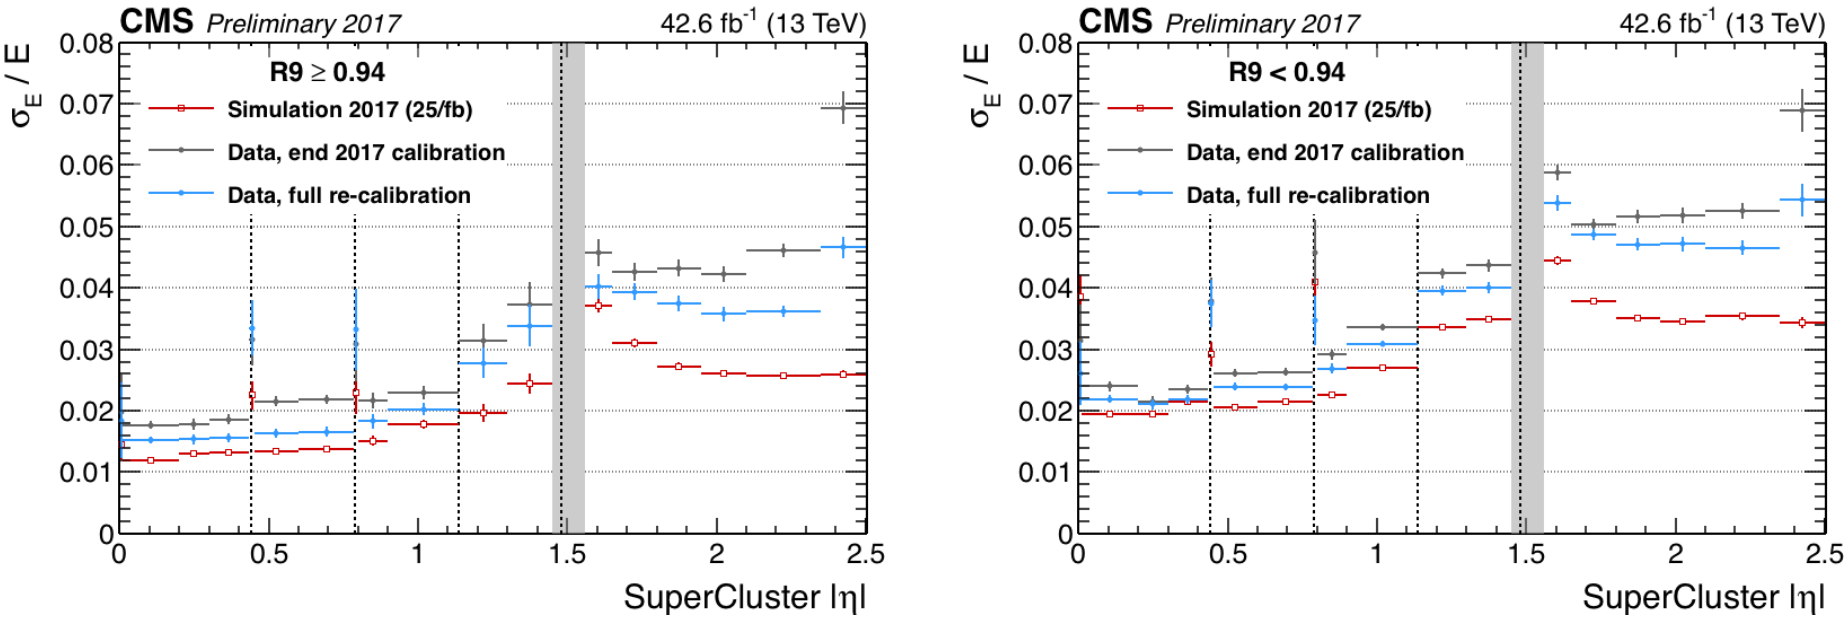
\includegraphics[width=1.0\linewidth]{Figures/chapter2_Figure/ecal_energy_resolution_2017.png}
\caption{CMS ECAL energy resolution.}
\label{Fig:CMS_ECAL_energy_resolution}
\end{center}
\end{figure}

%For the future challenges of higher luminosity LHC from Run 3 and so on, ECAL of CMS is undergoing through 
%%start from page 36
%
%
\subsection{Hadron Calorimeter (HCAL)}
It is the part of CMS detecting system, which helps for the detection and as well as energy measurements of strongly interacting particles such as quarks (or the ones in composition of quarks), gluons hadronic jets (like neutrons, pions and etc.). 
Being hermetic, HCAL also helps to measure missing transverse energy (MET) which can be associated to invisible particles like neutrinos which is important studies like top quark production.
%CMS being a general purpose detector is capable to study several final state signatures involved in a large range of high energy processes. The hadron 
%calorimeter (HCAL) provides the measurement of energies and positions of hadronic jets (for example neutrons, protons, kaons and 
%pions )\cite{cms:HCALTDR}. HCAL being hermetic is also 
%helpful to calculate MET that can be assigned to neutrinos or other invisible particles. 
HCAL assembles with CMS system between the solenoid magnet and ECAL as can be seen in the Fig. ~\ref{Fig:CMS_detector_design} at radial distance from 1.77 m to 2.95 m.
Benefitting from pretty short interaction length, at most brass is chosen as absorber throughout the HCAL. Brass is a non-magnetic low cost material.
HCAL provides pseudorapidity coverage upto $|\eta| < $ 3.0 beyond which, 11.2 m away from the interaction point, froward Hadron Calorimeter (HF) is employed on both sides of the detector providing additional coverage upt $|\eta| < $ 5.2. HF helps to detect particles from proton-proton collisions emerging at very small angles with respect the beam axis. \par
Schematic diagram of HCAL is shown in the Figure ~\ref{Fig:CMS_HCAL_layout} ~\cite{Reference34}.

\begin{figure}
\begin{center}

\includegraphics[width=0.7\linewidth]{Figures/chapter2_Figure/CMS_HCAL.pdf}
\caption{CMS HCAL layout.}
\label{Fig:CMS_HCAL_layout}
\end{center}
\end{figure}

HCAL is splitted into barrel and endcap regions, HB and HE which give pseudorapidity coverage of $|\eta|<1.33 $ and HE of $1.3 < |\eta| < 3$ respectively.

%There are no gaps or cracks in HCAL to make sure 
%to capture all known particles, leaving MET with only possibility of escaped particles. It is fitted 
%between ECAL and the CMS solenoid at radial distance from 1.77 m to 2.95 m providing a coverage of pseudorapidity up to $|\eta| < $ 3.0, beyond
%this point a forward hadron calorimeter (HF) is installed at a distance of 11.2 m from the collision point on both ends extending pseudorapidity coverage 
%to $|\eta| < $ 5.2. As HCAL is placed inside 3.8 T of magnetic field, so absorber is chosen to be a material which is non-magnetic. Also, due to requirement on maximum number
%of interaction length, cost and mechanical property brass has been chosen for CMS HCAL.
\par HCAL is also splitted into barrel and encap regions, HB and HE respectively. HB consistes of 32 towers provides coverage of pseudorapidity of $|\eta|<1.4 $ and HE of $1.3 < |\eta| < 3$. This results in 2304 towers in a segmentation of $\Delta \eta \times \Delta \phi $ = 0.87 \times 0.87. 
% to be continued

HB serves as a single longitudinal sampling readout. 
HB is split into two halves (HB${}^{+}$ and HB${}^{-}$) which consist of 36 similar wedges each weighing 26 tonnes made up of brass plates. %illustrated in Figure \ref{Fig:CMS_HCAL_layout}. The 
%wedges are built with the absorbant, the plane brass plates kept along beam axis. All plates are made of brass with physical properties described in 
%Table \ref{Tab:CMS_HCAL_bras_properties} except inner and 
%outer most made of steel for structural strength. Table \ref{Tab:HCAL_absorber_thickness} shows the thickness of each layer. 
It may happen that tail of showers of hadrons which leak from rear of calorimeters may penetrate into ECAL and/or magnet. Therefore, additional calorimeter called Hadron Outer (HO) is installed outside the solenoid that used the coil of the magnet as absorber. With this effective thickness of HCAL becomes above 10 interaction lengths. HO has scintillator of 10 mm thickness and helps to improve resolution of HCAL for MET.\\
Pseudorapidity coverage of $3 < |\eta| < 3$ is provided by sub part of HCAL whihc is called Hadron Forward (HF). It suffers huge flux of the particles due to which sampling material is required to be hard against the radiations. For this purpose, steel/quartz fibre was used. HF is located 11.2 away from interaction point with 1.65 m absorber depth. With the incident particle flux, Cerenkov radiations are emitted through quartz fibers which is then channeled to photomultipliers (PMs).

HCAL is constructed with alternate layers of plastic and brass (the absorber and scientillator respectively) which helps to measure the arrival time, position and energy of a particle. 
Plates of brass are 79 mm thick each with 99 mm gaps for the scintillators installation.  
%Optical fibers collect all the light emitted
When a particle passes through scintillator, optical fibers collect the emitted lights and pass it to readout box. i
Total energy is calculated by summation of the light over many layers in depths
called tower. The scintillator in HCAL are arranged in the from of 70,000 tiny tiles. 
%individual tiles makes scintillator tray by grouping them in $\phi$ layers to limit the number of readout boxes.  These trays works as individual units, so it
%can be replaced or tested easily. 
%Rather than single-particle energy resolution, design of HCAL endcap was more motiviated from the goal that cracks between to minimize the cracks between barrel and endcaps regions of HCAL rather than energy resolution of single-particle. 
%\subsubsection{Forward Calorimeter}
%The two HF are placed on both sides of CMS to catch up the particle emerging from proton- proton collisions at very small angle relative to beam axis as shown
%in Figure \ref{Fig:CMS_HCAL_layout}~\cite{Reference34}. HF 
%is most forward region of the detector where enormous particle fluxes are expected. 
%On average, the energy deposited in HF only is 8 times more as compared to the whole CMS detector. The design of HF calorimeter for such harsh conditions was a
%considerable challenge. With integrated luminosity of $5 \times 10^{5}$~\ipb at $|\eta| = 5$, HF will absorb a radiation dose of about 10 MGy. The rate of charged hadrons is also extremely high. 
%Because of hard conditions HF material and design is different from rest of the HCAL. 
%\begin{figure}
%\begin{center}
%
\includegraphics[width=0.7\linewidth]{Figures/chapter2_Figure/CMS_HCAL.pdf}
%\caption{CMS HCAL layout.}
%\label{Fig:CMS_HCAL_layout}
%\end{center}
%\end{figure} 
%\begin{table}
%\caption{Properties of brass of HCAL.}
%\label{Tab:CMS_HCAL_bras_properties}
%\begin{center}
%\begin{tabular}{|c|c|}
%  \hline 
%  chemical composition & 70\% Cu, 30\% Zn \\ \hline 
%  density (g/cm${}^{3}$)& 8.53  \\ \hline
%  radiation length (cm) & 1.49 \\ \hline
%  interaction length (cm) & 16.42 \\ \hine
%  \hline
%\end{tabular}
%\end{center}
%\end{table}
%\begin{table}
%\caption{HCAL absorber thickness.}
%\label{Tab:HCAL_absorber_thickness}
%\begin{center}
% \begin{tabular}{|c|c|c|}
%  \hline
% layer type & material composition & thickness (mm) \\ \hline
%  front plate & steel & 40 \\ \hline
%  1-8 & brass & 50.5 \\ \hline
%  9-14 & brass & 56.5 \\ \hline
%  back plate & steel & 75 \\ \hline
%\end{tabular}
%\end{center}
%\end{table}
\par The energy resolution of the HCAL (i.e. HB, HO and HE) is given as
\begin{equation}
 %\left(\frac{\sigma}{E}\right)^{2}= \left(\frac{90\%}{\sqrt{E}}\right)^{2}+(4.5\%)^2        
 \left(\frac{\sigma}{E}\right)^{2}= \left(\frac{90\%}{\sqrt{E}}\right)^{2}+(a)^2        
\end{equation}
and for that of HF it is given as
\begin{equation}
 %\left(\frac{\sigma}{E}\right)^{2}= \left(\frac{170\%}{\sqrt{E}}\right)^{2}+(9.0\%)^2.        
 \left(\frac{\sigma}{E}\right)^{2}= \left(\frac{170\%}{\sqrt{E}}\right)^{2}+(b)^2.        
\end{equation}

Where $a$ and $b$ are constants having values 0.045 and 0.09 repectively.


There were subsequent upgrades in HCAL during Run 2 era. In 2017, PMTs were replaced with new multi-anode PMTs and additionally electronics replaced for better differentiation of real hit from the muons which hit the PMT window.  
In 2017, HE of HCAL was upgraded and photo detectors were replaced with latest silicon photo multipliers (SiPMs) for noise elimination and better photo detection efficiency ~\cite{pixel_hcal_upgrade}. %(reference in comments) % https://cms.cern/news/cms-prepares-pixel-and-hcal-upgrades
%\subsection{Superconducting Magnet}
%The CMS central is superconducting solenoid~\cite{cms:MFTDR,Reference36,Reference37,Reference38} designed to have bore of diameter 6 m and length 12.5 m producing magnetic 
%field of 3.8 T which is 100,000 time stronger than earth magnet.  The CMS solenoid is the largest ever built magnet weighs 12,000 tonnes, powerful 
%enough in providing a strong magnetic field in its dimensions throughout the detector. It surrounds CMS ITS, ECAL and HCAL. i
%The task of the magnetic field
%is to efficiently bend the charged particles when they more throught it. More the momentum of the charged particles less they bend, so high energetic charged particles require a stronger magnetic field for its momentum to be measured accurately. CMS aims to have excellent momentum resolution with such 
%strong magnetic field specially for muons. 
%The CMS magnetic is made of coil of NbTi wire which supplies the uniform magnetic field when current 
%pass through it. The NbTi becomes superconductor at $-268.5^{\circ}$~C (4~K) which allows a huge amount of current (10,000~A) to pass through it. To maintain
%this temperature liquid helium is used. A large bending is achieved in tacker by stronger magnetic field providing precise and efficiencies momentum measurement. 
%The magnetic field direction inside (tracker) and outside the solenoid (muon system) allows to make second momentum measurement for muons. 
%% \begin{table}
%% \begin{center}
%% \label{Tab:CMS_HCAL_bras_properties}
%% \caption{Parameters of CMS Magnet.}
%%  \begin{tabular}{|c|c|}
%%  \hline
%%  \multicolumn{2}{|c|}{General parameters} \\ \hline
%%  Length of magnet & 12.5~m \\
%%  Diameter of cold bore & 6.3~m \\
%%  Central induced magnetic field & 4~T \\
%%  Total Ampere-turns & 41.7 MA-turns \\
%%  Nominal current & 19.14~kA \\
%%  Inductance & 14.2~H \\
%%  Energy stored & 2.6~GJ \\ \hline
%%  \end{tabular}
%% \end{center}
%% \end{table}
\subsection{CMS Muon System }
Identification of muons originating from the collision point is a great challenge. Having long lifetime (i.e. 2.19 \times $10^{-6}$ ~which is even higher in relativitic regime), they tend to cross the whole detector without decaying. Also, having higher mass (about 200 times the mass of electrons) it tends to lose very little energy via bremsstrahlung. So, they leave track however they deposit very little amount of energy in the calorimeters. Hence a dedicated muon system was proposed and installed as outermost sub-detector of CMS. It is benefitted from three different strategies for detection and measurements on  muons. 

\begin{itemize}
	\item Drift Tubes (DT), only in barrel region
	\item Cathode Strip Chamber (CSC), only in endcap region
	\item Resistive plate chamber (RPC), in barrel and endcap regions both % esift Tubes (DT), only in barrel region
\end{itemize}

Muon identification in the CMS detector is provided by its outer most layer of sub-detector called muon system~\cite{cms:muonsystem_TDR}. The detection of the muons is very important for many physics
process. In particular, for SM Higgs boson decay to $ZZ/ZZ^{*}$ which is labeled as a golden channel if each Z boson decays to a pair of opposite charged muons. Best 
best mass resolution can be obtained with four muons in final state as muons are less effected  by detector material as compared to electrons because they 
interact  weakly with detector material. Along with this example, SUSY and other model for new physics searches also encourages the necessity for their
reconstruction of muons with excellent resolution.
\par To have a robust and precise muon system was one of the core motive of CMS as indicated by  detector name. Identification, triggering and momentum
measurement of the muons are the tasks assigned to  the muon system. The flux-return yoke and strong magnetic field are playing crucial role for excellent 
muons momentum resolution and triggering. The flux-return yoke by absorbing the hadrons helps for muons identification.
\par Muon system was essentially designed as cylindrical shape to provide full pseudorapidity coverage with detection area of 25000~m${}^{2}$, having 
barrel and  endcaps regions. Muons detection is  based on gasses detectors of three types. The strength of magnetic field is uniform in barrel region with less 
neutron-induced background. Drift tubes are installed providing pseudorapidity coverage $|\eta| < 1.2$, as illustrated in Figure \ref{Fig:CMS_muon_system_layout}. The barrel region is arranged to have four muons
station, measuring $r-\phi$ bending plane and  distance along beam side. The arrangement of the drift cells are offset by the half of the width of cell 
providing dead spot in efficiency, determination of standalone bunch crossing and excellent time resolution by utilizing mean timer circuits. The direction
and number of chambers are optimized to get maximum efficiency of combination of the hits from different stations to get single track which is helpful to 
reject the background. In endcap region, where non-uniform strength of magnetic field and more background is expected cathode strip chambers (CSCs) are installed
that providing coverage $ 0.9 < |\eta| < 2.4$. Like DT, there 4 CSCs stations on each endcap. Each station is composed of chambers, which are capable to work
independently, aligned perpendicularly to z-axis and spread between the flux-return plates. In order to overcome uncertainties of background rates and 
assignment of correct bunch crossing number, resistive plate chambers (RPCs) are planted both in the barrel and the endcap detector regions. There is a dedicated trigger
system for each type of muons gasses detector including RPCs. Good time resolution, fast response and coarser spatial resolution makes RPCs distinct from 
CSCs and DT. The RPCs also plays vital role for the combination of multiple hits in a chamber to for tracks. The RPCs are installed in between DT and CSCs in  
region the barrel and the endcap region respectively.
\begin{figure}
\begin{center}
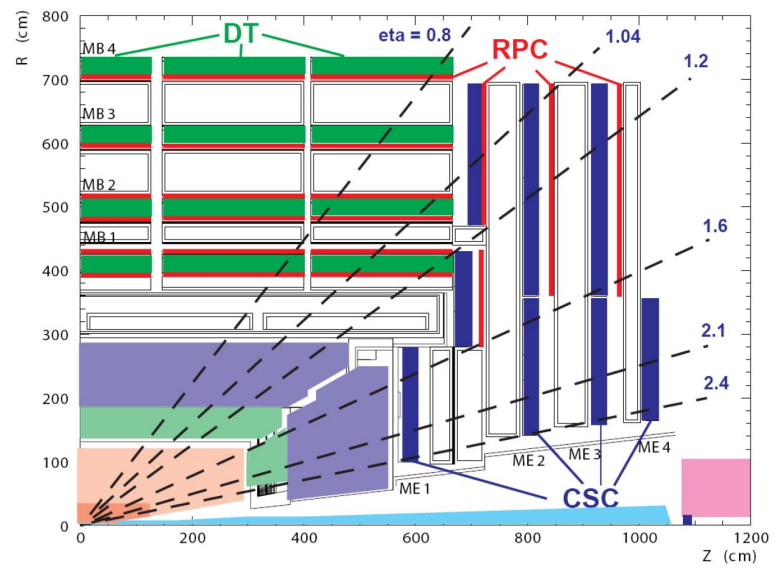
\includegraphics[width=0.7\linewidth]{Figures/chapter2_Figure/MS_layout.png}
\caption{CMS muon system layout.}
\label{Fig:CMS_muon_system_layout}
\end{center}
\end{figure} 

%\subsubsection{Drift Tubes of muon system of CMS}
%The DTs are planted in the barrel region of CMS muon system that provides pseudorapidity coverage of $|\eta| < 1.2 $ as illustrated
%in Figure \ref{Fig:CMS_muon_system_layout}. Whole DT system consists of 5 wheels 
%along z-axis, and 4 stations along radial direction (MB1, MB2, MB3, MB4). Each station is build with 12 chambers except fourth which contains 14 chambers. Each drift
%chamber of an average size of 2m$\times$2.5m  is made of 12 aluminium layers, making 3 groups of four. The central group provides the coordinates 
%measurement along z-axis and other two groups measures $r-\phi$. There are about 60 drift tubes in each chamber, each 4~cm wide made of drift cells each
%of size 42~mm~$\times$~13~mm. The 50$\mu$m wire made of stainless steel serves as anode while two ``I-shaped`` aluminum tape each of thickness 50$\mu$m 
%are  cathodes of the drift cell as shown in Figure \ref{Fig:CMS_DT_electric_field}. As any charges particle pass by the drift cell,  it ionizes the gas by 
%removing electrons from its atom. This establish a electric field finishing of at positively charged wire.  Distance between the  wire and the muon 
%track is estimated by drift time of these electrons.  The cell is filled with mixture of CO${}_{2}$ (15\%) Ar (85\%) gases which is 
%inexpensive and safe. Other qualities of this mixture are good saturation drift velocity (5.4~cm/$\mu$s) and quenching. To keep 
%drift velocity steady, the filled gas is kept at a constant pressure inside the chambers. The pressure in each wheel is continuously monitored by sensors. 
%It is expected to inject 10\% new gas everyday.
%
%\begin{figure}
%\begin{center}
%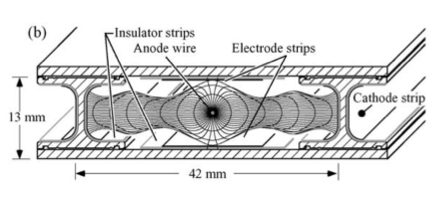
\includegraphics[width=0.7\linewidth]{Figures/chapter2_Figure/dt.png}
%\caption{DT electric field created by cathode, anode and insulating strips .}
%\label{Fig:CMS_DT_electric_field}
%\end{center}
%\end{figure} 
%\subsubsection{Cathode Strip Chambers of the CMS muon system}
%The cathode strip chambers (CSC) are installed at endcap region of CMS muon system providing the coverage of pseudorapidity upto $|0.9| < |\eta| < 2.4$, 
%illustrated in Figure \ref{Fig:CMS_muon_system_layout}. In the endcap regions, the strength of magnetic field
% is non-uniform which forced to use in endcap some different technology from the barrel region. Another challenge for CSCs is  higher 
%expected neutron-induced background as compared to the barrel region. The endcaps of the muon systems are made up of 468 CSCs arranged in four station like the
%barrel region
%(ME1, ME2, ME3 and ME4). The pseudorapidity range from $|0.9| < |\eta| < 1.2$ is covered by both CSCs and DTs. The chambers are aligned trapezoidal, each chamber
%is covering 10${}^{\circ}$ or 20${}^{\circ}$ in $\phi$. RPCs are also installed between CSCs stations.
%\par A single chamber is the basic unit which capable to work independently which is shown in Figure \ref{Fig:CMS_CSC_layout}. The CSC is multiple wire detector
%made of 6 layers of positively 
%charged anode interleaved with 7 layers of negatively charged cathode wires made of cooper filled within gas volume as shown in Figure \ref{Fig:CMS_CSC_layout}. The
%cathode and 
%anode wires are at right angle to each other and provides two position coordinates of each particle. As the charged particle pass through chamber, it will 
%ionize the gas atoms producing avalanche of electrons to anode wires, illustrated in Figure \ref{Fig:CMS_CSC_layout_ef} . As the wires are 
%nearby, CSCs not only provides excellent momentum resolution  but 
%helps to trigger the event as well. It feeds $r-\phi$ resolution of 2~mm to first level trigger, $75\mu$m %off-line spatial resolution in $r-\phi$ 
%for ME1/1 and ME1/2 chambers and $150\mu$m for other stations. The CSCs also help to assign bunch crossing with an efficiencies of 92\% which can be enhanced 
%up to 99\% by simple majority out of all chambers. CSC has tendency to operate at high event rates and in an environment where the strength of magnetic field is non-uniform. This makes CSCs robust which does not require precise
%gas pressure and temperature. Multilayer CSCs is useful for the combination of  hits in CSCs and tracker detectors.
%%%%%%%
%\begin{figure}[!htb]
%  \begin{center}
%    \subfigure[]{
%      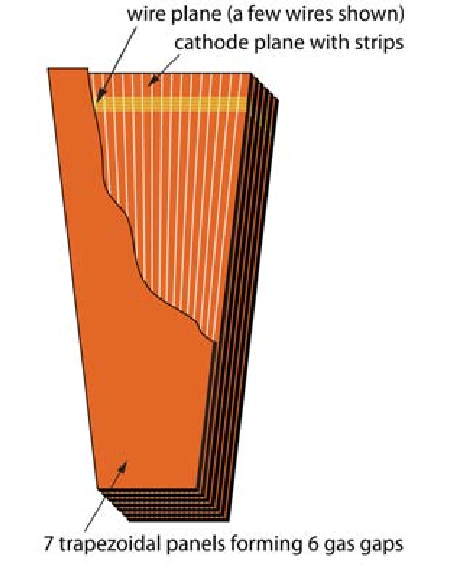
\includegraphics[width=0.48\textwidth,angle=0]{Figures/chapter2_Figure/csc_layout.png}
%      \label{Fig:CMS_CSC_layout}
%    }
%    \subfigure[]{
%      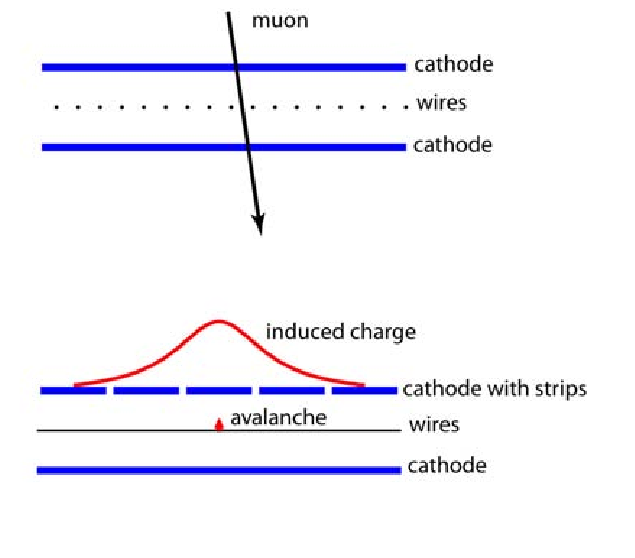
\includegraphics[width=0.48\textwidth,angle=0]{Figures/chapter2_Figure/csc_principle.png}
%      \label{Fig:CMS_CSC_layout_ef}
%    } 
%    \caption{CSC layout (left) and induced current (right) when a charged particle pass thorugh it .}
%  \label{fig:CSC_test_2}
%\end{center}
%\end{figure}
%
%%=============
%%============
%\subsubsection{Resistive Plate Chambers of muon system of CMS}
%RPCs are important part of CMS muon system installed in both barrel and endcap region. Time resolution of RPCs is excellent which is their main motivation. Additionally, spatial resolution of RPCs is also good. These  very fast responsive detector providing another muon trigger along with CSCs and DTs. RPCs are capable to provide 
%a time resolution of about a nano-second.
%\par RPCs are made of two high resistive plastic positive and negative charged plates, kept parallel to each other, with gas filled inn between them. The 
%gas mixture consists of 95\% of $C_{2}H_{2}F_{4}$ and 5\% of $C_{4}H_{10}$. As the muon pass through the RPCs, electrons librated during primary and secondary ionization of the gas  create
%avalanche which is received by outer metallic strips with a short but precise delay in time. Quick momentum measurement is feeded to trigger the event. The RPCs excellent time resolution assign bunch crossing 
%with ultimate precision.
%\subsubsection{Momentum Resolution}
%CMS detector is capable to measure muons transverse momentum independently by  using tracker or muon system. The expected transverse momentum resolution of muons system
%has been studied for the using muons of $p_{T} = 40$~GeV from Z and W boson decays and found to be 10\%(20\%) in barrel and endcap regions. Global muons can 
%also be reconstructed at CMS by the combining the information from tracker and muons system. As compared to muon system, tracker gives better resolution for muons $p_T$ less than 100~GeV and vice versa. The transverse momentum resolution is found to be improved sufficiently by using global 
%muons i.e 1\%(2\%) for $p_{T} < 100$~GeV in barrel(endcap) regions.
%For muons with $p_{T}$  greatar than 100~GeV, transverse momentum resolution of CMS muon system improves upto 8\% and 10\% in the barrel and endcap regions respectively. 
%Momentum 
%resolution of CMS muon system alone, tracker alone and combination of both are shown in Figure \ref{Fig:CMS_muon_momentum_resolution}~\cite{cms:muonsystem_TDR_2}.
%\begin{figure}
%\begin{center}
%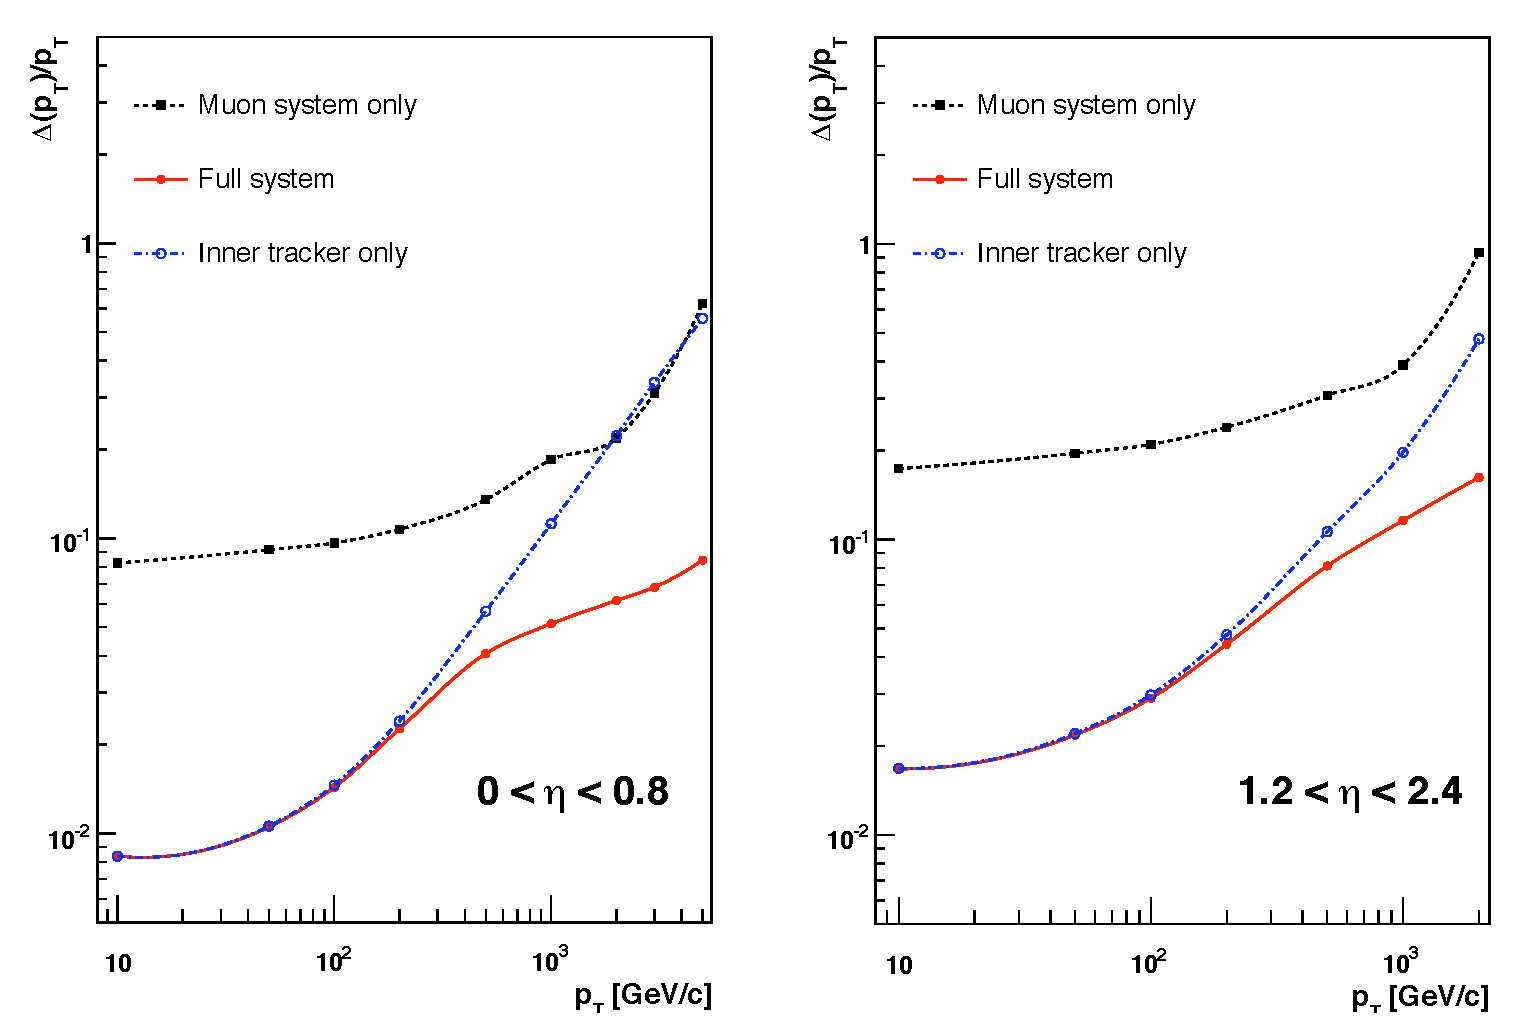
\includegraphics[width=0.7\linewidth]{Figures/chapter2_Figure/muon_resol.pdf}
%\caption{Momentum resolution of muon as a function of $p_T$ of muons both in barrel and endcap regions.}
%\label{Fig:CMS_muon_momentum_resolution}
%\end{center}
%\end{figure} 
%\subsection{Trigger and Data Acquisition System of CMS}
%The LHC running at its nominal parameters provides particle collisions produced with frequency of 40~MHz. Most of these events are soft collisions and uninteresting for new physics as they 
%are like minimum bias collisions. Though CMS detector is capable to reconstruct all of these events but storing all these events will fill the CMS storage in days. 
%So trigger system of CMS helps of select interesting events out of all for further steps. The events which does not pass the first step trigger are deleted permanently. 
%Trigger system performs the first step for physics event selection which reduces the event rate from  40~MHz down to ~1kHz into two layers Level-1 and the high-level
%triggers (shortly written as L1 and HLT respectively).
%\par The L1 trigger is made of the programmable electronics, dropping the event rate drastically to 100~kHz. To be fast, L1 trigger events by their energy and momentum calculations
%estimated by only using coarse in muon system and calorimeter instead of complete high resolution information. The L1 trigger decides to select or reject event in 3.2$\mu$m.   
%\par All events with positive L1 decision, with their complete information, are transferred to HLT which makes use of one thousand commercial processors. It uses
%the growing complex algorithms which exploit high details of the event. Decision time of HLT varies with event number with mean time of about $50$~ms. 
%Since HLT has excess of complete information of an event, it demands a greater bandwidth of the order of 1Tb/s.
%\par For example, to look for Higgs boson decay into 4-leptons final state, the trigger would look for energetic leptons in the detector. For L1 trigger, electron and muons 
%points to a narrow energy deposit in ECAL and hit pattern in tracker and the muon system respectively. While for HLT, momentum and total energy of the leptons 
%are reconstructed by ECAL and combination of muon system and inner tracker.
%\subsubsection{Level-1 Trigger Architecture}
%Configuration of L1 trigger is elaborated in Figure \ref{Fig:CMS_L1_trigger_configuration}. It can be classified into calorimeter 
%and muon triggers. Each ECAL and HCAL has independent regional trigger feeding to global calorimeter trigger. Similarly, muon 
%trigger has local triggers for each sub-detector merging into global muon trigger. Finally, global calorimeter and muon triggers merge into global trigger which
%makes L1 final decision.
%\par Each local trigger feeds to global/regional trigger by providing trigger primitives groups (TPGs) based on coarse of sub-detector. Regional calorimeter trigger (RCT)
% builds objects which deposit their energy in ECAL and HCAL such as jets, $\gamma$, electrons, photons and tau's.  Similarly, in muon triggering, DT/CSC/RPC track finders
% feeds muons tracks to muon global trigger (MGT). Global muon and calorimeter trigger feeded four best candidates at most, which are then sent to global trigger (GT).
% GT compares these candidates with L1 trigger menu to decide weather to keep to reject the event. Some triggers in the  menu evolved  with increasing LHC center
% of mass energy by tightening the requirement on candidate or  pre-scaled (selecting only the nth event) to control the output rate. Candidates 
% able to fire at least one trigger out of whole trigger menu is kept for further investigation by HLT. For example, the trigger/bit ``L1 SingleEG8Iso'' in the L1 trigger 
% menu requires one isolated (candidate with zero or little hadronic activity around it) electron or photon at least with $p_{T}$ greater than 8~GeV. 
%\begin{figure}
%\begin{center}
%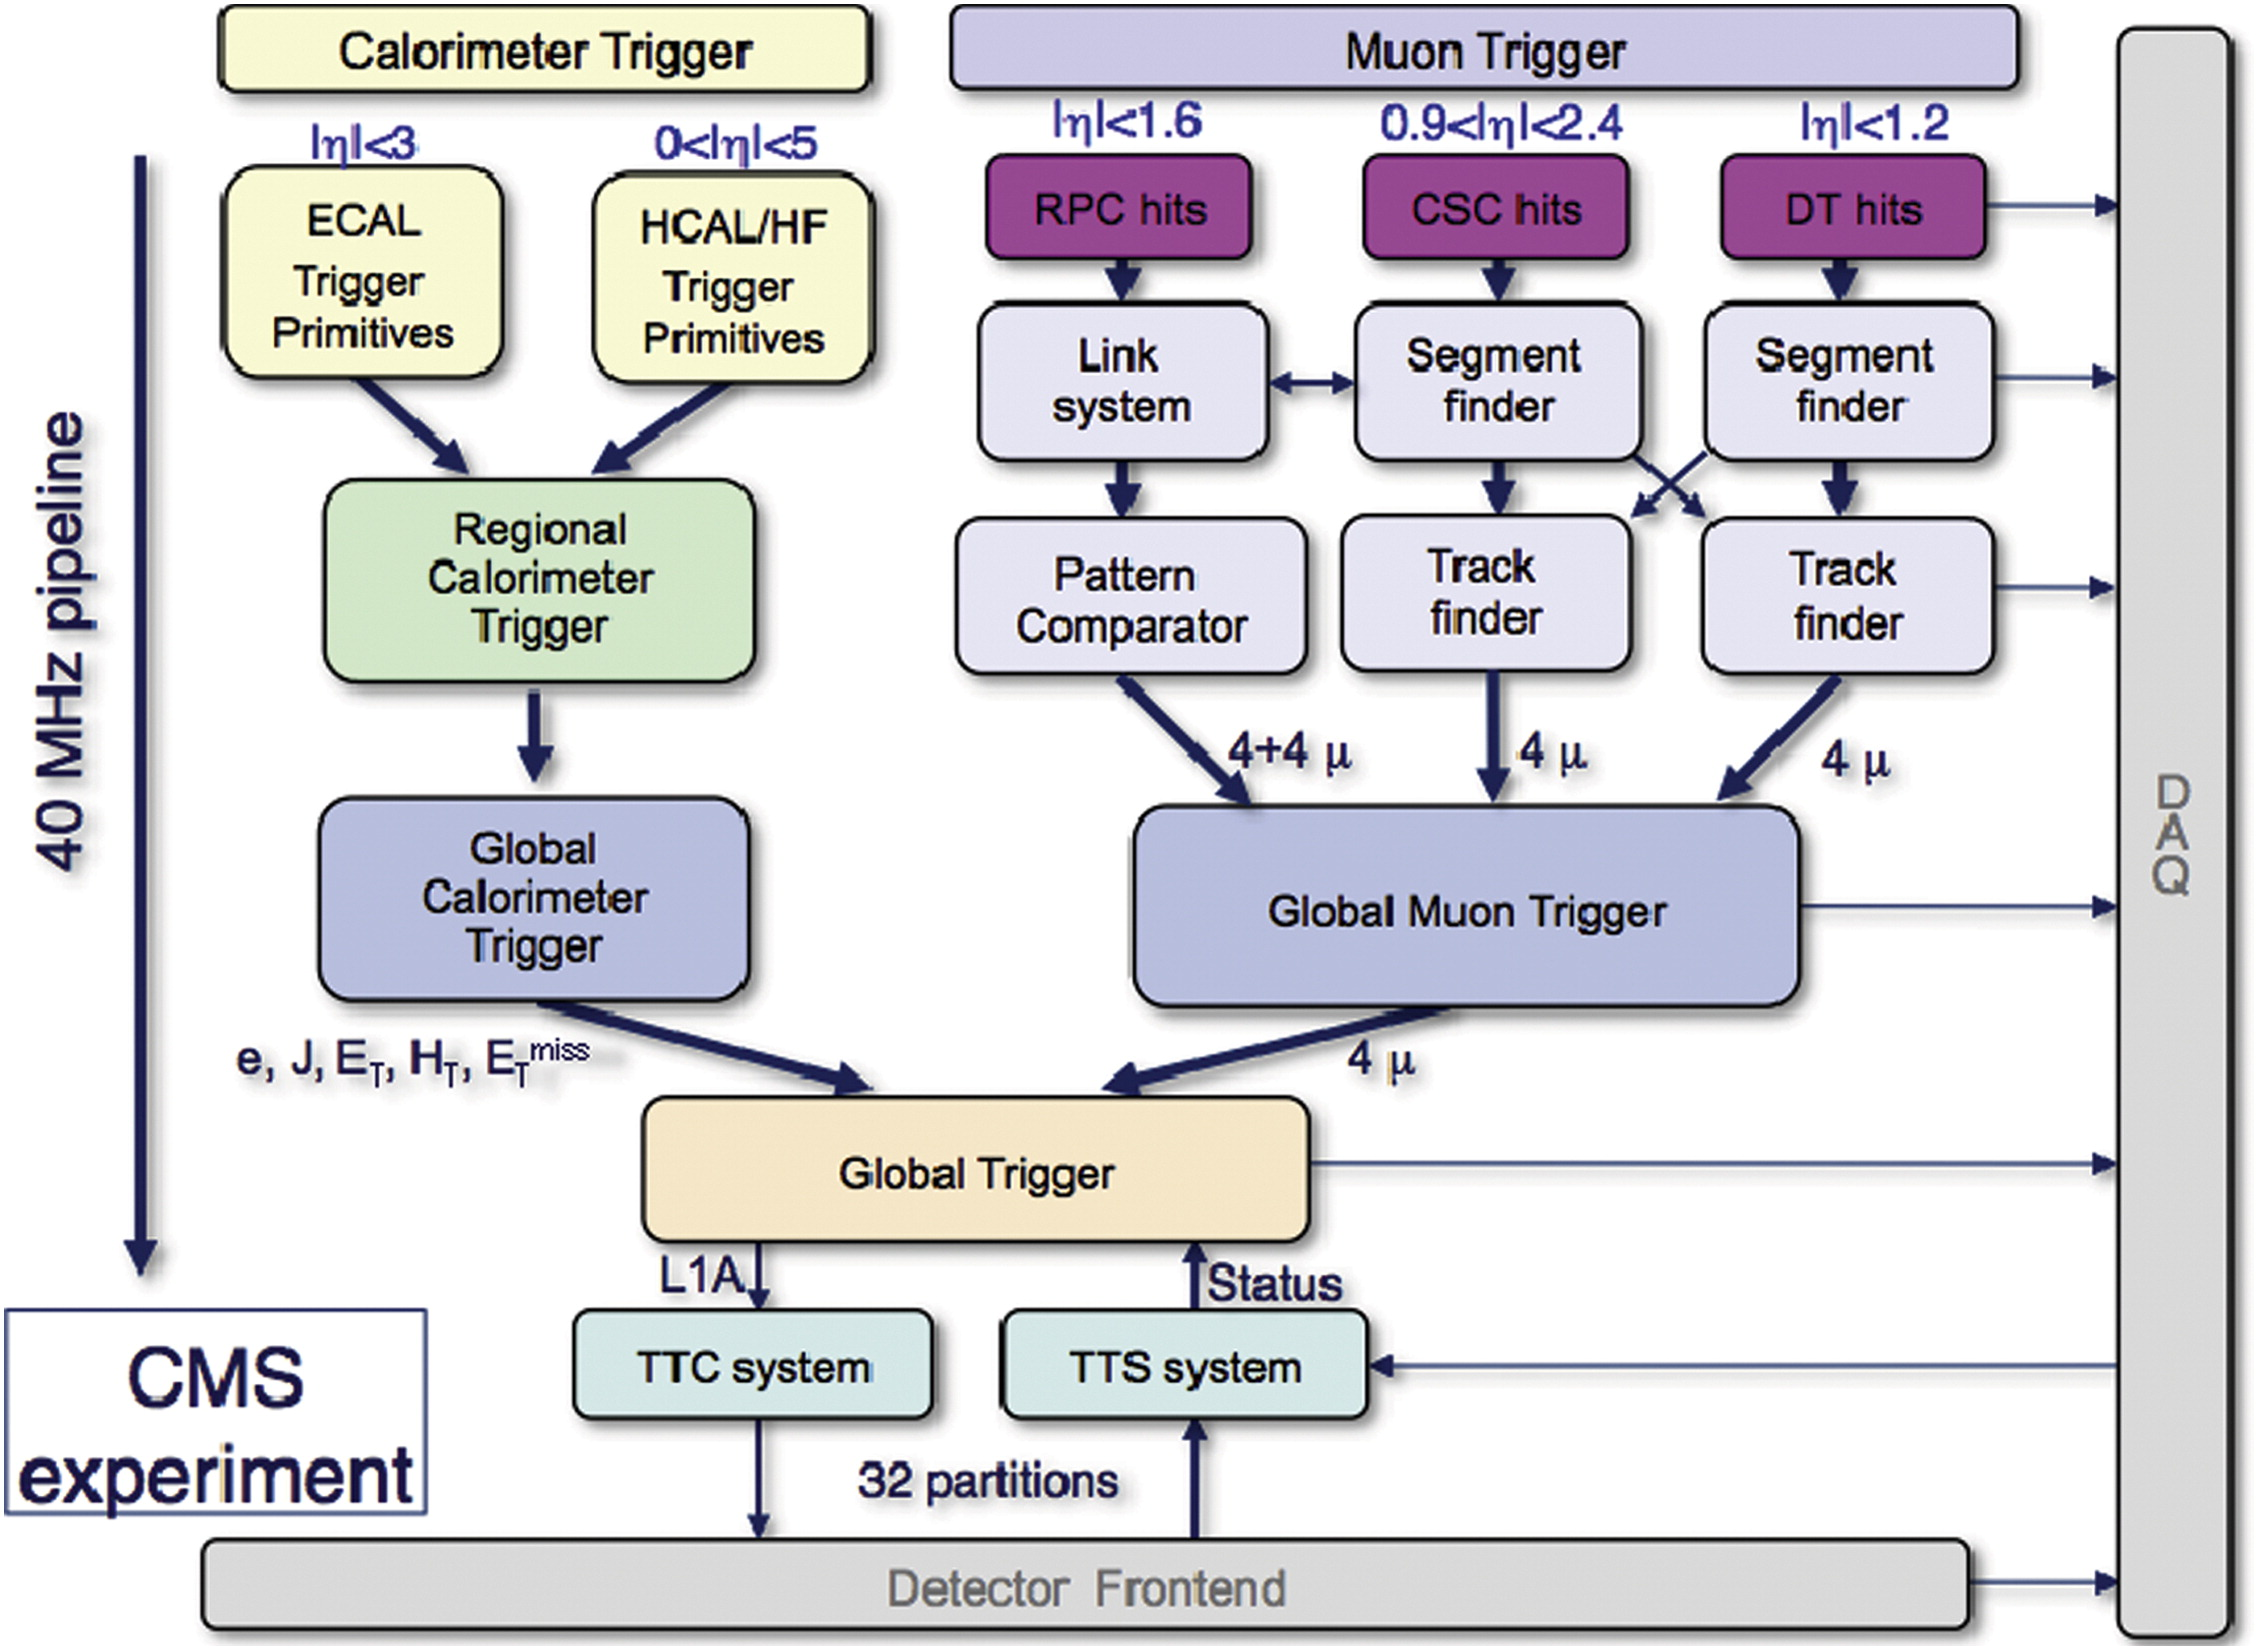
\includegraphics[width=0.7\linewidth]{Figures/chapter2_Figure/L1_new.jpg}
%\caption{The configuration of L1 trigger.}
%\label{Fig:CMS_L1_trigger_configuration}
%\end{center}
%\end{figure} 
%\subsubsection{High-Level Trigger Architecture}
%HLT  is three level (2, 2.5 and 3) trigger with growing complexity starting at level 2  which usually works on top of the information provided by L1 trigger. Goal of the HLT is to use output event rate of L1-trigger(100kHz) and reduce it upto 1 kHZ.  Level 2 HLT is to build fine granularity objects by combining the information from sub-detectors e.g from preshower and ECAL energy clusters are combined for electrons. Bremsstrahlung  
%of the electrons causes its energy to spread into several neighbor cells. To compensate this effect, clusters of ECAL are combined to form superclusters.
%\par At HLT level 2.5, the inner tracker information is combined and matched with calorimeters and muon system. In case of electron, energy supercluster is 
%matched with the hits in the tracker, if matches it form a seed. Tracker hits are matched with the hits in muon system to reconstruct global muon.
%HLT level 3 reconstructs the complete track, if its found electron seed or matching hits of muon. After these three stages, precise energy and momentum are calculated of 
%the objects that decides to accept or reject the event. 
%\par There are more than 200 different HLT paths each derived by at least one L1 bit. The data which pass the HLT trigger is organized into different 
%datasets according to the objects reconstructed in the event and the passed selection e.g an event with two muons reconstructed with transverse momentum
%greater than 8 and 17~GeV will be placed in "DoubleMu'' dataset. 
%\subsubsection{Data Acquisition (DAQ) System of CMS}
%The schematic skeleton of CMS DAQ system is presented in Figure \ref{Fig:CMS_DAQ_layout}. CMS DAQ provides data from 650 different readout channels to 
%HLT along with enough computing resources to limit the output data rate~\cite{cms:DAQ_TDR}. Frangments of an event with a size of 2KB is provided by each module. 
%In order to read data from detector sensors, Front End Drivers (FEDs) utilizea network whose bandwidth is 100 Gb/s.  These FEDs are located underground
%at the level of the detector called counting room. Events are then transferred to a system where these are filtered at 100 kHz rate maximum. The complete reconstruction
%of the objects of the event and high machine luminosity is the reason for this high rate.
%\begin{figure}
%\begin{center}
%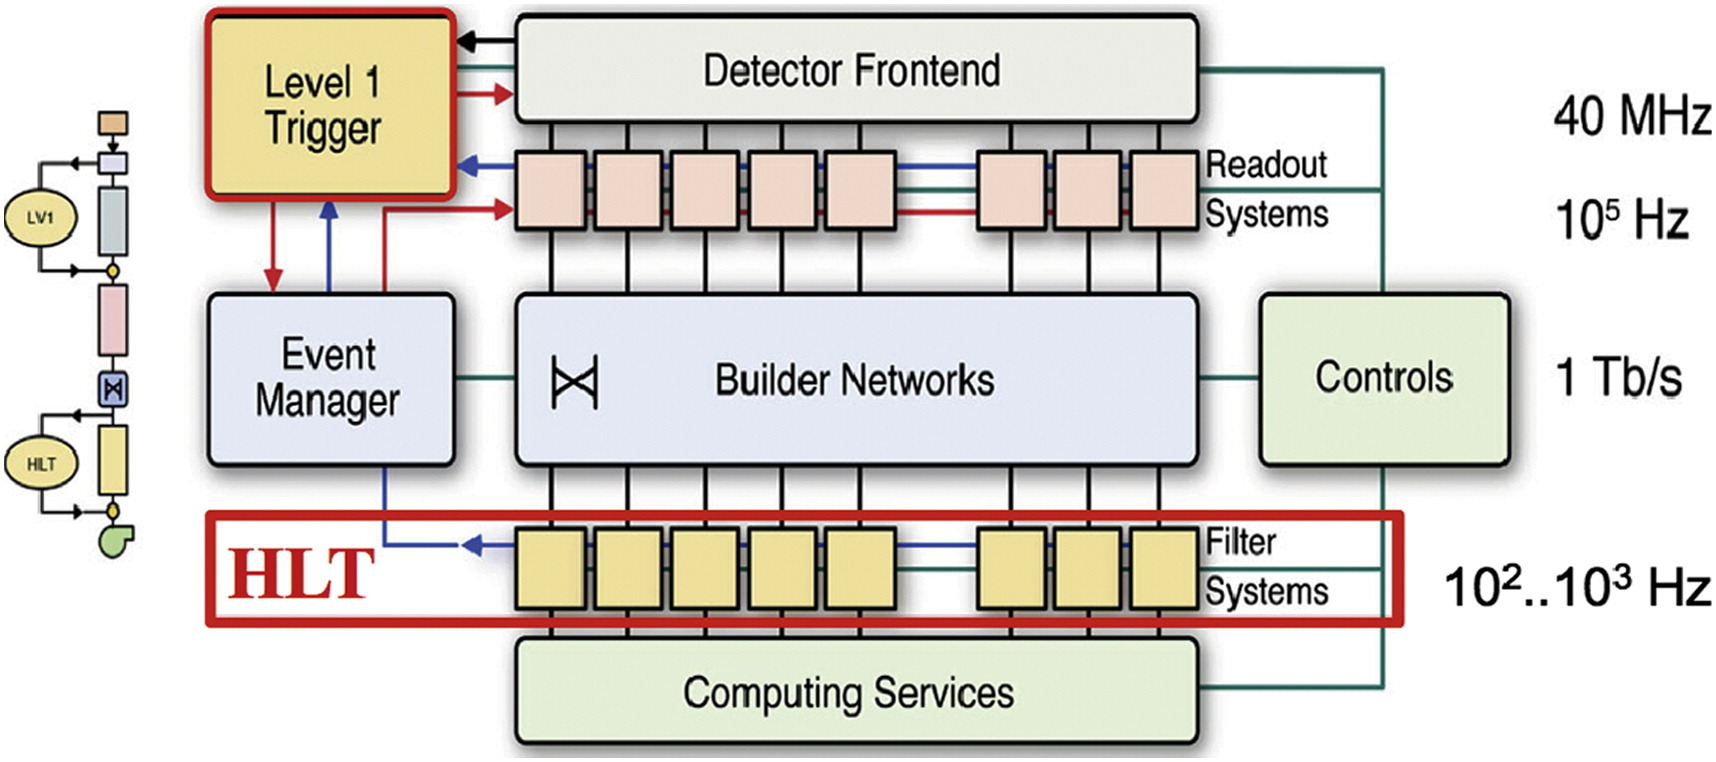
\includegraphics[width=0.7\linewidth]{Figures/chapter2_Figure/daq_new.jpg}
%\caption{The CMS DAQ system structure.}
%\label{Fig:CMS_DAQ_layout}
%\end{center}
%\end{figure}
%%\subsection{Computing Grid}
%%An important and last step after data collection is to process it with full detailed reconstruction algorithms and made available for physics analysis.Although,  
%%trigger system of CMS drastically reduces the amount of data but even then CMS delivers data at the order of petabytes every year.  To analyze and store this huge 
%%amount of the data, LHC has connected huge number of computing resources from collaborative institutes or universities, computer centers and middleware providers 
%%through a grid known as the Worldwide LHC Computing Grid (WLCG). 
%%\par There are three layers of Tier (Tier-0, Tier-1 and Tier-2) for data flow between different computing sites. 
%%The types of dataset is described below briefly
%%\begin{itemize}
%% \item RAW data that contains all the recorded information from detector along with triggers decisions and other metadata. A copy of RAW data is achieved and placed
%% at permanent storage element. A occupancy of  around 1.5 (2.0) MB/event is needed to store data (simulated data) in RAW version.
%% \item Many algorithms and pattern recognition techniques like cluster and track-finding; primary and secondary vertex reconstruction etc. are applied to RAW data to 
%% obtain RECO data format. RECO events occupancy is roughly three times less than RAW (0.5~MB/event).
%% \item The most compact format of data AOD (analysis object data) is obtained by dropping unnecessary information and reducing per event size up to 100 KB.
%%\end{itemize}
%%Tier-0 is located at CERN with which copies the recorded data to permanent storage, promptly reconstruct data from RAW version to have first version of
%%prompt-RECO data and copies RAW data to Tier-1 centers. Tier-1 are mainly held in national computing centers and labs from collaborative countries. 
%%At each Tier-1, a fraction of detailed the reconstruction of RAW data simulated data has been performed to get AOD. Tier-1 also responsible to store and 
%%export AOD format data to Tier-2. The last layer Tier-3 is hosted by CMS collaborative institutes where main analysis activity, alignment, detector related studies and 
%%offline calibration is done. Tier-3 are used for Monte Carlo (MC) data production which can be exported to Tier-1 for long term storage.
